\documentclass[survey]{cpecmu}

%% This is a sample document demonstrating how to use the CPECMU
%% project template. If you are having trouble, see "cpecmu.pdf" for
%% documentation.
\usepackage{enumitem}
\setlist[itemize,2]{label=\textcolor{black}{\large$\circ$}}

\projectNo{S047-1}
\acadyear{2025}

\titleTH{ระบบสนับสนุนการตัดสินใจสำหรับการวางแผนระบบขนส่งสาธารณะ}
\titleEN{DeSS-T : Decision Support System for Public Transit Planning}

\author{นางสาวปวีณนุช เพราะสุนทร}{Paweennut Prohsoontorn}{650610783}
\author{นายอนุวัตร เอี่ยมศรี}{Anuwat Aeamsri}{650610819}
\author{นางสาวอิศวรา คงศรีเจริญ}{Issawara Kongsricharoen}{650610821}

\cpeadvisor{paskorn}
\cpecommittee{santi}
\cpecommittee{navadon}


%% Some possible packages to include:
\usepackage[final]{graphicx} % for including graphics

%% Add bookmarks and hyperlinks in the document.
\PassOptionsToPackage{hyphens}{url}
\usepackage[colorlinks=true,allcolors=Blue4,citecolor=red,linktoc=all]{hyperref}
\def\UrlLeft#1\UrlRight{$#1$}

%% Needed just by this example, but maybe not by most reports
\usepackage{afterpage} % for outputting
\usepackage{pdflscape} % for landscape figures and tables. 
\usepackage{float}
%% Some other useful packages. Look these up to find out how to use
%% them.
% \usepackage{natbib}    % for author-year citation styles
% \usepackage{txfonts}
% \usepackage{appendix}  % for appendices on a per-chapter basis
% \usepackage{xtab}      % for tables that go over multiple pages
% \usepackage{subfigure} % for subfigures within a figure
% \usepackage{pstricks,pdftricks} % for access to special PostScript and PDF commands
% \usepackage{nomencl}   % if you have a list of abbreviations

%% if you're having problems with overfull boxes, you may need to increase
%% the tolerance to 9999
% \tolerance=9999

\bibliographystyle{plain}
% \bibliographystyle{IEEEbib}

% \renewcommand{\topfraction}{0.85}
% \renewcommand{\textfraction}{0.1}
% \renewcommand{\floatpagefraction}{0.75}

%% Example for glossary entry
%% Need to use glossary option
%% See glossaries package for complete documentation.
\ifglossary
  \newglossaryentry{lorem ipsum}{
    name=lorem ipsum,
    description={derived from Latin dolorem ipsum, translated as ``pain itself''}
  }
\fi

%% Uncomment this command to preview only specified LaTeX file(s)
%% imported with \include command below.
%% Any other file imported via \include but not specified here will not
%% be previewed.
%% Useful if your report is large, as you might not want to build
%% the entire file when editing a certain part of your report.
% \includeonly{chapters/intro,chapters/background}

\begin{document}
\maketitle
\makesignature

\ifproject
\begin{abstractTH}
เขียนบทคัดย่อของโครงงานที่นี่

การเขียนรายงานเป็นส่วนหนึ่งของการทำโครงงานวิศวกรรมคอมพิวเตอร์
เพื่อทบทวนทฤษฎีที่เกี่ยวข้อง อธิบายขั้นตอนวิธีแก้ปัญหาเชิงวิศวกรรม และวิเคราะห์และสรุปผลการทดลองอุปกรณ์และระบบต่างๆ
\enskip อย่างไรก็ดี การสร้างรูปเล่มรายงานให้ถูกรูปแบบนั้นเป็นขั้นตอนที่ยุ่งยาก
แม้ว่าจะมีต้นแบบสำหรับใช้ในโปรแกรม Microsoft Word แล้วก็ตาม
แต่นักศึกษาส่วนใหญ่ยังคงค้นพบว่าการใช้งานมีความซับซ้อน และเกิดความผิดพลาดในการจัดรูปแบบ กำหนดเลขหัวข้อ และสร้างสารบัญอยู่
\enskip ภาควิชาวิศวกรรมคอมพิวเตอร์จึงได้จัดทำต้นแบบรูปเล่มรายงานโดยใช้ระบบจัดเตรียมเอกสาร
\LaTeX{} เพื่อช่วยให้นักศึกษาเขียนรายงานได้อย่างสะดวกและรวดเร็วมากยิ่งขึ้น
\end{abstractTH}

\begin{abstract}
The abstract would be placed here. It usually does not exceed 350 words
long (not counting the heading), and must not take up more than one (1) page
(even if fewer than 350 words long).

Make sure your abstract sits inside the \texttt{abstract} environment.
\end{abstract}

\iffalse
\begin{dedication}
This document is dedicated to all Chiang Mai University students.

Dedication page is optional.
\end{dedication}
\fi % \iffalse

\begin{acknowledgments}
Your acknowledgments go here. Make sure it sits inside the
\texttt{acknowledgment} environment.

\acksign{2020}{5}{25}
\end{acknowledgments}%
\fi % \ifproject

\contentspage

\ifproject
\figurelistpage

\tablelistpage
\fi % \ifproject

% \abbrlist % this page is optional

% \symlist % this page is optional

% \preface % this section is optional


\pagestyle{empty}\cleardoublepage
\normalspacing \setcounter{page}{1} \pagenumbering{arabic} \pagestyle{cpecmu}

\chapter{\ifenglish Introduction\else บทนำ\fi}

% นิยาม environment mypara สำหรับย่อหน้าใหม่หลัง section
\newenvironment{mypara}{\par\setlength{\parindent}{1em}\indent}{}


% กำหนดให้ย่อหน้าอัตโนมัติ
\setlength{\parindent}{2em}

\section{\ifenglish Project rationale\else ที่มาของโครงงาน\fi}
\begin{mypara}
    \indent การออกแบบระบบขนส่งสาธารณะโดยรถบัสเป็นงานที่ซับซ้อน เนื่องจากต้องคำนึงถึงความหลากหลายของโครงข่ายเส้นทาง 
    สภาพแวดล้อมทางกายภาพ ความหนาแน่นของประชากร \\ 
    \indent โดยเฉพาะในบริบทของมหาวิทยาลัยเชียงใหม่ ระบบขนส่งสาธารณะมีความซับซ้อนเป็นพิเศษ 
    เนื่องจากต้องให้บริการครอบคลุมทั้ง คณะ อาคารเรียน และหอพักนักศึกษา โดยมีจุดรับ-ส่งมากถึง 56 ป้าย ครอบคลุม 9 เส้นทางหลัก 
    ขณะที่นักศึกษามีการเปลี่ยนอาคารเรียนตามช่วงเวลา การใช้รถบัสไฟฟ้ายังเพิ่มข้อจำกัดด้านระยะทางและเวลาวิ่งต่อรอบ 
    ส่งผลให้การกำหนดเส้นทางและความถี่ในการให้บริการมีความท้าทายยิ่งขึ้น \\
    \indent ด้วยความซับซ้อนดังกล่าว การใช้แบบจำลองจึงเป็นเครื่องมือสำคัญในการออกแบบและวิเคราะห์ระบบขนส่ง 
    โดยช่วยจำลองเส้นทางที่หลากหลาย จำลองความถี่ของการออกรถ วิเคราะห์ข้อมูลที่จำเป็น เพื่อช่วยให้ผู้วางแผนสามารถตัดสินใจได้อย่าง
    แม่นยำและมีประสิทธิภาพมากขึ้น  \\
    \indent โปรแกรมจำลอง ในปัจจุบันส่วนใหญ่ไม่ได้ถูกออกแบบมาเพื่อระบบขนส่งสาธารณะโดยเฉพาะ \\
    แม้ว่าจะสามารถนำไปประยุกต์ใช้กับระบบขนส่งสาธารณะได้ในบางกรณี แต่การใช้งานจริงกลับค่อนข้างยุ่งยากและซับซ้อน 
    เนื่องจากโปรแกรมเหล่านั้นไม่ได้ถูกพัฒนาขึ้นเพื่อรองรับความต้องการเฉพาะของงานนี้ตั้งแต่ต้น โดยเฉพาะอย่างยิ่งกับระบบขนส่งสาธารณะ
    ประเภทรถบัส ซึ่งมีความซับซ้อนในเรื่องของเส้นทาง เวลาเดินรถ และความจุผู้โดยสารที่แตกต่างจากระบบขนส่งรูปแบบอื่นๆ 
    จึงทำให้โปรแกรมจำลอง ในปัจจุบันยังไม่สามารถตอบโจทย์การวางแผนและบริหารจัดการระบบขนส่งรถบัสได้อย่างมีประสิทธิภาพ
\end{mypara}

\section{\ifenglish Objectives\else วัตถุประสงค์ของโครงงาน\fi}
\begin{enumerate}
    \item เพื่อออกแบบและพัฒนาระบบจำลองระบบขนส่งสาธารณะประเภทรถบัสที่สามารถวิเคราะห์ข้อมูลที่เกี่ยวข้อง เช่น อัตราการใช้งานของรถบัส เวลารอโดยเฉลี่ยของผู้โดยสาร และอัตราการเกิดเหตุการณ์ที่รถบัสมีการใช้งานเกินเวลาหรือระยะทางที่กำหนด
    \item เพื่อให้ระบบจำลองที่พัฒนาขึ้นมีความแม่นยำและถูกต้องตามสถิติและสอดคล้องกับเหตุการณ์ที่เกิดขึ้นจริง 
    \item เพื่อออกแบบและพัฒนาปรับปรุงระบบให้สอดคล้องกับความต้องการของผู้ใช้งานจริง
\end{enumerate}

\section{\ifenglish Project scope\else ขอบเขตของโครงงาน\fi}

\subsection{\ifenglish Software scope\else ขอบเขตด้านซอฟต์แวร์\fi}
    \begin{mypara}
        \indent ระบบถูกออกแบบเพื่อใช้จำลองข้อมูลจากตารางการเดินรถ โดยอาศัยข้อมูลสถิติในอดีตเป็นหลัก 
        ไม่ได้อ้างอิงจากข้อมูลแบบ Real-time ทั้งนี้ระบบสามารถประยุกต์ใช้งานได้กับระบบรถ 
        Shuttle Bus โดยทั่วไป ไม่จำกัดว่าต้องพื้นที่ใดพื้นที่นึงเท่านั้น
    \end{mypara}
\subsection{\ifenglish Hardware scope\else ขอบเขตด้านฮาร์ดแวร์\fi}
    \begin{mypara}
        \indent ผู้ใช้งานสามารถเข้าถึงระบบผ่านเครื่องคอมพิวเตอร์ส่วนบุคคล (PC หรือ Laptop)
         โดยยังไม่รองรับการใช้งานผ่านอุปกรณ์พกพา (Mobile Device)
    \end{mypara}
\subsection{\ifenglish Data scope\else ขอบเขตด้านข้อมูล\fi}
    \begin{mypara}
        \indent ระบบใช้ข้อมูลจากตารางการเดินรถและข้อมูลเชิงสถิติย้อนหลังมาเป็นฐานในการวิเคราะห์และจำลองสถานการณ์ 
        โดยในกรณีศึกษานี้จะมุ่งเน้นที่ระบบขนส่งมวลชนภายในมหาวิทยาลัยเชียงใหม่ จำนวน 2 สายบริการ
    \end{mypara}
\subsection{\ifenglish User scope\else ขอบเขตด้านผู้ใช้งาน\fi}
    \begin{mypara}
        \indent ระบบสามารถรองรับการใช้งานพร้อมกันได้หลายบุคคล (Multi-user) 
        กลุ่มผู้ใช้งานหลักประกอบด้วยผู้ดูแลระบบ ผู้วางแผนการเดินรถ และผู้บริหารที่เกี่ยวข้อง
    \end{mypara}

\section{\ifenglish Project constraints\else ข้อจำกัดของโครงงาน\fi}

\subsection{\ifenglish Time constraint\else ข้อจำกัดด้านเวลา\fi}
    \begin{mypara}
        \indent ข้อมูลบางประเภทได้มาจากการเก็บรวบรวมจากผู้ใช้จริง ซึ่งอาจทำให้เกิดช่วงเวลาที่ไม่สะดวกต่อการดำเนินการเก็บข้อมูล 
        นอกจากนี้ ระยะเวลาในการดำเนินโครงงานมีเพียง 1 ปี จึงอาจทำให้รายละเอียดบางประการของซอฟต์แวร์เกิดข้อผิดพลาดหรือคลาดเคลื่อนได้
    \end{mypara}
\subsection{\ifenglish Equipment constraints\else ข้อจำกัดด้านอุปกรณ์\fi}
    \begin{mypara}
        \indent จำนวนรถที่ให้บริการภายในมหาวิทยาลัยเชียงใหม่มีบางส่วนที่อยู่ในสภาพชำรุด 
        ส่งผลให้จำนวนรถที่ใช้งานจริงอาจแตกต่างจากข้อมูลที่นำมาใช้ในการจำลอง (Simulation) 
        ซึ่งอาจก่อให้เกิดความคลาดเคลื่อนของผลลัพธ์ นอกจากนี้ ยังมีโอกาสที่รถบางคันออกให้บริการไม่เป็นไปตามตารางเวลา 
        ส่งผลให้ผลลัพธ์จากการจำลองอาจไม่ตรงกับสภาพความเป็นจริงเช่นกัน
    \end{mypara}

\section{\ifenglish Expected outcomes\else ประโยชน์ที่ได้รับ\fi}
    \begin{mypara}
        \indent ระบบจำลองจะช่วยสนับสนุนการตัดสินใจในการนำตารางการเดินรถไปประยุกต์ใช้จริงได้อย่างมีประสิทธิภาพและเหมาะสมมากยิ่งขึ้น
    \end{mypara}
\section{\ifenglish Technology and tools\else เทคโนโลยีและเครื่องมือที่ใช้\fi}

\subsection{\ifenglish Software technology\else เทคโนโลยีด้านซอฟต์แวร์\fi}
    \begin{mypara}
        \indent โครงงานนี้ใช้เทคโนโลยีด้านซอฟต์แวร์และเครื่องมือดังนี้ ส่วนของ Display Frontend ใช้ Vite และ TypeScript 
        สำหรับการพัฒนา UI/UX และการโต้ตอบ พร้อมทั้งใช้ Leaflet.js สำหรับการแสดงผลแผนที่ ส่วนของ Logical Model 
        ใช้ Python ร่วมกับ FastAPI โดยอาศัย Salabim ในการสร้างและควบคุมกระบวนการจำลอง และใช้ SciPy (fitcurve) 
        สำหรับการวิเคราะห์เชิงคณิตศาสตร์ ในส่วนต่อมา API Controller ใช้ Go fiber สำหรับการจัดการการยืนยันตัวตน 
        การเชื่อมต่อและบริหารจัดการฐานข้อมูล การกำหนดเส้นทาง API และการจัดการคำร้องขอ 
        ส่วน Database ใช้ PostgreSQL เพื่อการจัดเก็บและบริหารข้อมูล นอกจากนี้ ในส่วนของ 
        Infrastructure ใช้ Docker สำหรับสร้างสภาพแวดล้อมที่สม่ำเสมอและง่ายต่อการปรับใช้งาน และใช้ DigitalOcean 
        สำหรับโฮสต์ระบบและให้บริการออนไลน์
    \end{mypara}


\section{\ifenglish Project plan\else แผนการดำเนินงาน\fi}

\begin{plan}{6}{2025}{2}{2026}
    \planitem{6}{2025}{6}{2025}{ระบุและนิยามปัญหา}
    \planitem{7}{2025}{7}{2025}{ระบุ Stakeholder}
    \planitem{8}{2025}{8}{2025}{User Study}
    \planitem{8}{2025}{10}{2025}{ศึกษาหลักการที่เกี่ยวข้อง}
    \planitem{8}{2025}{10}{2025}{กำหนดวิธีการแก้ปัญหา}
    \planitem{9}{2025}{10}{2025}{การออกแบบ Userflow และ Wireframe}
    \planitem{10}{2025}{11}{2025}{ออกแบบ UX/UI}
    \planitem{11}{2025}{1}{2026}{พัฒนา Prototype แรก}
    \planitem{11}{2025}{1}{2026}{การเก็บรวบรวมข้อมูลสำหรับการทดสอบแบบจำลอง}
    \planitem{1}{2026}{2}{2026}{การทดสอบและการเก็บ Feedback จากผู้ใช้งานจริง}
    \planitem{1}{2026}{2}{2026}{พัฒนาและปรับปรุงซอฟแวร์}
\end{plan}

\section{\ifenglish Roles and responsibilities\else บทบาทและความรับผิดชอบ\fi}
\begin{mypara}
    \indent ในการทำโครงงานนี้สมาชิกแต่ละคนมีบทบาทและหน้าที่ที่รับผิดชอบดังนี้
\end{mypara}
\begin{enumerate}
    \item \textbf{นางสาวปวีณนุช เพราะสุนทร รหัส 650610783} มีบทบาทเป็น Project Owner และ Developer 
    โดยรับผิดชอบการกำหนดขอบเขตงานให้ตรงความต้องการของระบบ ออกแบบและพัฒนา Logical Model ที่เป็นส่วนของ Backend 
    และรับผิดชอบการพัฒนาและดูแล API Controller เพื่อเชื่อมต่อระหว่าง Frontend และ Backend
    \item \textbf{นายอนุวัตร เอี่ยมศรี รหัส 650610819} มีบทบาทเป็น Developer โดยรับผิดชอบการพัฒนาส่วน Display Frontend เพื่อให้ผู้ใช้สามารถโต้ตอบกับระบบได้ และดูแลการออกแบบและจัดการ 
    ฐานข้อมูล (Database) ให้มีโครงสร้างที่ถูกต้อง และสอดคล้องกับความต้องการของระบบ
    \item \textbf{นางสาวอิศวรา คงศรีเจริญ รหัส 650610821} มีบทบาทเป็น Developer และ Designer โดยรับผิดชอบการออกแบบและวางระบบ Infrastructure เพื่อสนับสนุนการทำงานภายในของระบบ 
    และออกแบบ UX/UI Design ให้เหมาะสมกับการใช้งานระบบ
\end{enumerate}
\section{\ifenglish%
Impacts of this project on society, health, safety, legal, and cultural issues
\else%
ผลกระทบด้านสังคม สุขภาพ ความปลอดภัย กฎหมาย และวัฒนธรรม
\fi}
\begin{mypara}
    \indent ด้านสังคม โครงงานนี้มีส่วนช่วยให้ผู้ใช้และผู้วางแผนนโยบายเข้าใจรูปแบบการเดินทางและพฤติกรรมการใช้ระบบขนส่งสาธารณะในชุมชนได้อย่างลึกซึ้งขึ้น โดยการวิเคราะห์ข้อมูลการเดินทางจริงร่วมกับการจำลองสถานการณ์ สามารถเห็นแนวโน้ม 
    เช่น ช่วงเวลาที่ผู้โดยสารหนาแน่น เส้นทางที่มีความต้องการสูง หรือพฤติกรรมการต่อคิวและขึ้นลงรถ ซึ่งข้อมูลเหล่านี้สามารถนำไปใช้ในการวางแผนและปรับปรุงเส้นทางรถ การจัดสรรรถและเวลาการเดินรถให้เหมาะสมกับความต้องการของผู้โดยสาร 
    ส่งผลให้ระบบขนส่งมีประสิทธิภาพมากขึ้น นอกจากนี้ยังช่วยยกระดับคุณภาพชีวิตของผู้คน เนื่องจากผู้โดยสารจะได้รับบริการที่สะดวก ปลอดภัย และลดเวลารอคอย อีกทั้งยังสนับสนุนการตัดสินใจด้านสังคม เช่น 
    การพัฒนาพื้นที่โดยรอบสถานีขนส่งและการกำหนดนโยบายส่งเสริมการใช้ขนส่งสาธารณะ

    \indent ด้านความปลอดภัย การใช้การจำลอง เป็นเครื่องมือสำคัญในการประเมินความเสี่ยงและทดสอบสถานการณ์ต่าง ๆ โดยไม่ต้องเสี่ยงต่อผู้ใช้งานจริง ตัวอย่างเช่น การตรวจสอบว่าการออกรอบแต่ละครั้ง 
    รถโดยสารสามารถวิ่งภายใต้ลิมิตเวลาที่กำหนดหรือไม่ หากเกินลิมิต อาจทำให้ระบบรถทำงานหนักจนดับ หรือเพิ่มความเสี่ยงต่อการเกิดอุบัติเหตุ การจำลองสถานการณ์เหล่านี้ช่วยให้สามารถวางมาตรการป้องกันล่วงหน้า 
    เช่น การปรับแผนรอบเดินรถ หรือการจัดสรรทรัพยากรให้เหมาะสม ส่งผลให้ระบบขนส่งสาธารณะมีความปลอดภัยและเชื่อถือได้มากยิ่งขึ้น

    \indent การปรับใช้เชิงวิศวกรรม การใช้การจำลองในเชิงวิศวกรรมช่วยให้สามารถออกแบบและปรับปรุงระบบขนส่งสาธารณะอย่างเป็นระบบและมีหลักวิศวกรรมรองรับ โดยสามารถนำข้อมูลจากการจำลองมาใช้ในการวิเคราะห์ปัญหาและออกแบบโครงสร้างการเดินรถ 
    และการบริหารจัดการทรัพยากรระบบรถ เพื่อให้รถทำงานได้อย่างปลอดภัยและมีประสิทธิภาพนอกจากนี้ การจำลองยังช่วยในการทดสอบสมมติฐานต่าง ๆ ก่อนนำไปใช้งานจริง ทำให้วิศวกรสามารถออกแบบมาตรการป้องกัน ปรับปรุงระบบ และวางแผนบำรุงรักษาได้อย่างเหมาะสม
\end{mypara}

\section{\ifenglish Project budget plan\else แผนการใช้งบประมาณ\fi}
\begin{enumerate}
    \item ค่าสมาชิกรายเดือนของ Canva Pro สำหรับการออกแบบเชิงกราฟิก\\
    \textbf{งบประมาณ:} 230 บาท/เดือน จำนวน 1 บัญชี เป็นเวลา 10 เดือน รวมเป็นเงิน 2300 บาท
    \item ค่าสมาชิกรายเดือนของ Overleaf สำหรับการเขียนเอกสาร \LaTeX \\
    \textbf{งบประมาณ:} 300 บาท/เดือน จำนวน 1 บัญชี เป็นเวลา 5 เดือน รวมเป็นเงิน 1500 บาท
    \item ค่าเช่ารายเดือนของ Droplet ผ่าน DigitalOcean สำหรับการพัฒนาและโฮสติ้งของระบบ\\
    \textbf{งบประมาณ:} 387 บาท/เดือน (2 GB / 1 CPU, 50 GB SSD Disk, 2 TB transfer) \\
    จำนวน 1 เครื่อง เป็นเวลา 5 เดือน รวมเป็นเงิน 1935 บาท
    \item ค่าเช่ารายเดือนของ Additional Storage ของ Droplet ผ่าน DigitalOcean สำหรับการ\\
    เก็บข้อมูล Workspace\\
    \textbf{งบประมาณ:} 162 บาท/เดือน ขนาด 50 GB เป็นเวลา 5 เดือน รวมเป็นเงิน 810 บาท
    \item ค่าโดเมนเนม .com ผ่าน Godaddy สำหรับการเข้าถึงระบบผ่านทาง URL ที่จดจำง่าย\\
    \textbf{งบประมาณ:} 400 บาท/ปี จำนวน 1 โดเมน รวมเป็นเงิน 400 บาท
    \item ค่าใช้จ่ายสำหรับการรวบรวมข้อมูลในการทดสอบระบบ\\
    \textbf{งบประมาณ:} 1500 บาท ตลอดการดำเนินโครงงาน
    \item ค่าอุปกรณ์สำนักงาน และการจัดทำโปสเตอร์\\
    \textbf{งบประมาณ:} รวมเป็นเงิน 1000 บาท
    \item ค่าใช้จ่ายสำหรับการเดินทาง(สมาชิกที่ไม่มีรถส่วนตัว)\\
    \textbf{งบประมาณ:} 600 บาท จำนวน 3 คน ตลอดการดำเนินโครงงาน รวมเป็นเงิน 1800 บาท\\ \\
    \textbf{งบประมาณรวมทั้งสิ้น:} 11255 บาท

\end{enumerate}
\chapter{\ifenglish Background Knowledge and Theory\else ทฤษฎีที่เกี่ยวข้อง\fi}

\section{บทนำ}
  \sloppy\indent ในบทนี้จะนำเสนอการศึกษาทฤษฎีและงานวิจัยที่เกี่ยวข้อง เพื่อเป็นแนวทางในการออกแบบและพัฒนาเว็บแอปพลิเคชันสำหรับระบบสนับสนุนการตัดสินใจในการวางแผนระบบขนส่งสาธารณะ 
  ระบบดังกล่าวถูกออกแบบให้ใช้การจำลอง (simulation) เพื่อสร้างสถานการณ์บนแผนต่างๆ 
  และให้ผลลัพธ์ใกล้เคียงกับความเป็นจริง ในบทนี้จะอธิบายแนวคิดและทฤษฎีที่เกี่ยวข้องกับการพัฒนาระบบดังกล่าว

\section{Platform Development}

\subsection{Frontend Display}
\subsubsection{Vite}
\indent Vite เป็น Frontend Build Tool และ Development Server ที่ออกแบบเพื่อปรับปรุงประสบการณ์การพัฒนาเว็บแอปพลิเคชันสมัยใหม่ มีจุดเด่นเรื่อง \textbf{ความเร็วสูง} และ \textbf{HMR (Hot Module Replacement) แบบเรียลไทม์} ทำให้การพัฒนา Frontend ราบรื่นและสนุกยิ่งขึ้น  

\begin{itemize}
    \item \textbf{Native ES Modules}: ใช้ฟีเจอร์ ES Modules ของเบราว์เซอร์ ทำให้ไม่ต้อง Bundle ทั้งโปรเจกต์ในระหว่าง Development
    \item \textbf{Instant Server Start}: เริ่ม Development Server ได้ทันทีโดยไม่ต้องรอ Build
    \item \textbf{Hot Module Replacement (HMR)}: เปลี่ยนแปลงโค้ดแล้วเห็นผลทันทีโดยไม่โหลดหน้าใหม่
    \item \textbf{Optimized Production Build}: ใช้ Rollup สำหรับสร้างไฟล์ Production ที่มีประสิทธิภาพและขนาดเล็ก
\end{itemize}

ในระบบสนับสนุนการตัดสินใจด้านขนส่งสาธารณะ Vite ถูกใช้เป็น Frontend Build Tool สำหรับ Next.js เพื่อพัฒนา Interface ที่โต้ตอบกับ Backend (Go Fiber) 
และแสดงผลข้อมูลเชิงพื้นที่/Simulation Model ดังนี้

\begin{enumerate}
    \item \textbf{Development Server และ HMR}
    \begin{itemize}
        \item พัฒนา UI/UX แบบ Interactive เช่น Map (Leaflet.js), Graph, และ Dashboard
        \item เปลี่ยนแปลงโค้ดแล้วเห็นผลทันที ทำให้ปรับ Layout หรือ Data Visualization ได้รวดเร็ว
    \end{itemize}
    
    \item \textbf{Integration กับ React / Next.js}
    \begin{itemize}
        \item ใช้ Vite เป็นเครื่องมือ Build สำหรับ Next.js/React Component
        \item จัดการ Asset, CSS Module, และ ES Modules ได้ง่าย  
        \item รองรับการทำ Code Splitting เพื่อลดขนาด Bundle และเพิ่ม Performance
    \end{itemize}
    
    \item \textbf{Data Fetching และ API Consumption}
    \begin{itemize}
        \item Frontend ติดต่อกับ Backend (Go Fiber) ผ่าน RESTful API  
        \item ดึงผลลัพธ์จาก Simulation Model หรือ PostGIS Spatial Query มาสร้าง Heatmap, Graph, หรือ Table แบบ Real-time
    \end{itemize}
    
    \item \textbf{Optimized Production}
    \begin{itemize}
        \item Build ไฟล์ Production ขนาดเล็ก, Tree-Shaking, และ Minification  
        \item ทำให้โหลดหน้าเว็บเร็วขึ้นแม้ข้อมูลเชิงพื้นที่หรือ Graph มีขนาดใหญ่
    \end{itemize}
\end{enumerate}

\subsubsection{TypeScript}
TypeScript เป็นภาษาโปรแกรมที่พัฒนาโดย Microsoft ซึ่งเป็น \textbf{superset ของ JavaScript} เพิ่มความสามารถด้าน \textbf{Static Typing} และ \textbf{Compile-Time Error Checking} ทำให้โค้ดมีความปลอดภัยและลดข้อผิดพลาดในระหว่างการพัฒนา  
\begin{itemize}
    \item \textbf{Static Typing}: ประกาศประเภทของตัวแปร, ฟังก์ชัน, และ Object ช่วยตรวจสอบข้อผิดพลาดก่อนรัน
    \item \textbf{Enhanced IDE Support}: รองรับ IntelliSense, Auto-completion, และ Refactoring
    \item \textbf{Compatibility}: สามารถรันโค้ด JavaScript ได้ทั้งหมด และ Compile เป็น JavaScript สำหรับ Browser หรือ Node.js
    \item \textbf{Object-Oriented Features}: รองรับ Class, Interface, Generics และ Module System
\end{itemize}

TypeScript ถูกใช้เป็นภาษาหลักในการพัฒนา Frontend ของระบบ ด้วย Next.js และ Vite Framework เพื่อสร้าง Interface ที่โต้ตอบกับ Backend (Go Fiber) และ Visualize ผลลัพธ์ของ Simulation Model / GIS Data
\begin{enumerate}
    \item \textbf{Static Typing for API Data}
    \begin{itemize}
        \item กำหนด Interface สำหรับ Response จาก Backend เช่น Simulation Result, Spatial Data
        \item ลดข้อผิดพลาดจากการเรียกใช้ JSON หรือ Object Property
    \end{itemize}
    
    \item \textbf{Component-Based Development}
    \begin{itemize}
        \item สร้าง React Component แบบ Typed เพื่อ Map, Graph, Table
        \item ใช้ Props และ State แบบ Type-Safe
    \end{itemize}
    
    \item \textbf{Improved Maintainability}
    \begin{itemize}
        \item ทำให้ทีมสามารถ Refactor โค้ดได้ง่ายและปลอดภัย
        \item รองรับการพัฒนา Feature ใหม่หรือปรับ UI/UX โดยไม่ทำลายระบบเดิม
    \end{itemize}
    
    \item \textbf{Integration with Vite / Next.js}
    \begin{itemize}
        \item Vite รองรับการ Compile TypeScript ได้โดยตรง
        \item TypeScript ช่วยให้การเชื่อมต่อ API, State Management, และ Component Interaction มีความปลอดภัยและมีประสิทธิภาพ
    \end{itemize}
\end{enumerate}

\subsection{Logical Model}
\subsubsection{Salabim}
Salabim เป็น Python-based Discrete-Event Simulation (DES) framework ที่ออกแบบมาเพื่อสร้างและรันระบบจำลองเชิงเหตุการณ์ (Event-Driven Simulation) ได้อย่างยืดหยุ่นและชัดเจน 
แนวคิดหลักของ Salabim ได้แก่:
\begin{itemize}
    \item \textbf{Discrete-Event Simulation}: ระบบเปลี่ยนแปลงสถานะเมื่อเกิดเหตุการณ์ (Event) เช่น การมาถึงของผู้โดยสาร การเคลื่อนที่ของรถ
    \item \textbf{Process-Oriented Modeling}: ใช้ Process class สำหรับกำหนดพฤติกรรมของ Entities (เช่น รถโดยสาร)
    \item \textbf{Resources}: สามารถกำหนด Resource, Queue, Priority Queue และเงื่อนไขการเข้าใช้
    \item \textbf{Stochastic Modeling}: สนับสนุนการสุ่มเหตุการณ์และเวลาในการรอ เช่น Arrival Time, Service Time
\end{itemize}

\subsubsection{แนวคิดดังกล่าวจะถูกนํามาประยุกต์ใช้ในระบบของเรา โดยใช้ใน Logical Model ดังนี้}
\begin{enumerate}
    \item \textbf{การจำลองเหตุการณ์ของผู้โดยสารและรถ}
    \begin{itemize}
        \item Entities: รถโดยสาร, ผู้โดยสาร, ป้ายรถ
        \item Events: Arrival, Departure, Boarding, Alighting
        \item Process: กำหนดพฤติกรรม เช่น รถวิ่งตามเส้นทาง, ผู้โดยสารขึ้น/ลง
    \end{itemize}
    
    \item \textbf{การจัดการทรัพยากร (Resource Management)}
    \begin{itemize}
        \item กำหนดจำนวนรถแต่ละเส้นทาง
        \item วิเคราะห์ปัญหาเวลารอของผู้โดยสาร
    \end{itemize}
    
    \item \textbf{การวิเคราะห์เชิงสถิติและผลลัพธ์}
    \begin{itemize}
        \item Collect Metrics: เวลาเฉลี่ยรอรถ, จำนวนผู้โดยสาร, ความหนาแน่น
        \item Visualization: ส่งผลลัพธ์ไปยัง Heatmap หรือ Graph ของ Frontend
        \item Scenario Analysis: ปรับจำนวนรถ, ตารางเวลา หรือเส้นทางเพื่อเปรียบเทียบประสิทธิภาพ
    \end{itemize}
\end{enumerate}

\subsection{API Controller}
% \subsubsection{Service-Oriented Architecture (SOA)}
% \indent แนวทางการออกแบบสถาปัตยกรรมระบบซอฟต์แวร์โดยแยกฟังก์ชันการทำงานของระบบออกเป็น 
% Services ที่เป็นอิสระจากกัน แต่สามารถสื่อสารและประสานงานกันได้ผ่านโปรโตคอลมาตรฐาน

% \begin{itemize}
%     \item \textbf{SOA} มุ่งเน้นการให้บริการ (Service) ในระดับองค์กร โดยมักจะใช้ ESB (Enterprise Service Bus) เป็นตัวกลาง
% \end{itemize}

% \indent แนวคิดดังกล่าวจะถูกนํามาประยุกต์ใช้ในระบบของเราโดยในโครงสร้างระบบ ดังนี้
% \begin{enumerate}
%     \item \textbf{API Controller (FastAPI)}  
%     ทำหน้าที่เป็น Gateway Service หรือ API Gateway เป็นจุดรับและส่งข้อมูล (Request/Response) จากผู้ใช้หรือระบบภายนอก รวมถึงทำ Authentication, Load Balancing
%     \item \textbf{Logical Model (Simulation/Calculation)}  
%     ทำหน้าที่เป็น Processing Service รับข้อมูลจาก API Controller เพื่อทำ Simulation หรือการคำนวณเชิงตรรกะ สามารถรันเป็น Service แยก เช่นบน Container (Docker) หรือ Serverless Function เพื่อเพิ่ม scalability ได้
%     \item \textbf{Frontend (Next.js / Vite)}  
%     สื่อสารกับ Backend ผ่าน REST API สามารถ deploy หรืออัปเดต UI ได้โดยไม่กระทบ backend
% \end{enumerate}

\subsubsection{RESTful API Design (Representational State Transfer)}
\indent รูปแบบการออกแบบ API สำหรับให้ระบบคอมพิวเตอร์สื่อสารกันผ่านเว็บ 
โดยแต่ละสิ่งที่ API จัดการจะถูกมองเป็นทรัพยากร (Resource) 
เช่น ข้อมูลผู้ใช้ ข้อมูล Simulation หรือเส้นทางเดินทาง โดยแต่ละทรัพยากรจะมี URL เฉพาะ 
และใช้ HTTP Methods (GET, POST, PUT, DELETE) เพื่อระบุการกระทำที่ต้องการกับทรัพยากรนั้น 
ระบบจะส่งข้อมูลกลับในรูปแบบที่อ่านง่าย เช่น JSON การใช้ RESTful API ช่วยให้ Frontend 
และ Backend แยกส่วนกันได้ชัดเจน เรียกใช้ Logic ที่ซับซ้อนผ่าน Request มาตรฐานได้ 
และทำให้การพัฒนาระบบง่ายต่อการเข้าใจ ใช้ซ้ำ และสเกลระบบได้ง่าย

\subsubsection{จากแนวคิดดังกล่าวจะถูกนํามาประยุกต์ใช้ในระบบของเราโดยจะมีประโยชน์ ดังนี้}
\begin{enumerate}
    \item \textbf{ความง่ายในการเข้าถึงและเข้าใจ}  
    URL และ HTTP Methods มีความเป็นธรรมชาติ และสอดคล้องกับมาตรฐานสากล ทำให้ทีมพัฒนาต่างๆ เข้าใจได้ง่าย
    \item \textbf{การทำงานแบบ Stateless}  
    แต่ละ Request เป็นอิสระ ช่วยให้ระบบสามารถ scale ได้ง่ายขึ้น โดยเฉพาะในสภาพแวดล้อม Cloud หรือ Container
    \item \textbf{การบูรณาการกับ Frontend/Backend}  
    Frontend (Next.js / Vite) สามารถเรียกใช้ Logic ที่ซับซ้อน (เช่น Simulation Model) ผ่าน API แบบมาตรฐานโดยไม่ต้องรู้รายละเอียดเชิงลึกของ Backend
    \item \textbf{สนับสนุนมาตรฐาน HTTP และเครื่องมือทั่วไป}  
    เช่น curl, Postman ทำให้การทดสอบและบันทึกเอกสารทำได้สะดวก
    \item \textbf{ความยืดหยุ่นในการพัฒนาและปรับปรุง}  
    สามารถเพิ่ม Endpoint ใหม่หรือเปลี่ยนแปลง Backend ได้โดยไม่กระทบกับ Client หากยังคง Interface เดิม
\end{enumerate}

\subsubsection{Go Fiber Framework}
\indent Go Fiber เป็น Web Framework สำหรับภาษา Golang ที่ได้รับแรงบันดาลใจจาก Express.js ของ Node.js มีจุดเด่นคือ ความเร็วสูง, น้ำหนักเบา และใช้งานง่าย เหมาะกับการสร้าง RESTful API, Microservices และ Web Application โดย Fiber ใช้ fasthttp เป็น HTTP engine ทำให้สามารถประมวลผล Request/Response ได้เร็วมากเมื่อเทียบกับ Framework อื่นๆ  

\subsubsection{คุณสมบัติเด่นของ Go Fiber ได้แก่:}
\begin{itemize}
    \item \textbf{Performance}: รองรับ Request จำนวนมากด้วย Latency ต่ำ  
    \item \textbf{Minimalism}: API เรียบง่าย เรียนรู้ง่ายและใกล้เคียงกับ Express.js  
    \item \textbf{Routing}: รองรับ Dynamic Routing, Group Routing, Middleware  
    \item \textbf{Middleware}: สามารถเพิ่ม Logging, CORS, Authentication, Compression, และอื่น ๆ  
    \item \textbf{WebSocket Support}: รองรับการสื่อสารแบบ Real-time  
\end{itemize}

\subsubsection{ประโยชน์ของ Go Fiber ในระบบของเรา}
\begin{enumerate}
    \item ความเร็วสูง ลดเวลา Response ของ API สำหรับ Simulation Model
    \item API เรียบง่ายและ Modular สามารถจัดการ Routing และ Middleware แยกตาม Module ได้
    \item รองรับการ Scale ระบบในอนาคต เช่น เพิ่ม Microservice หรือ Containerize ด้วย Docker
    \item ทำงานร่วมกับ Database และ Web GIS ได้อย่างราบรื่น
    \item สนับสนุนการพัฒนาแบบ Concurrent และ Real-time เช่น WebSocket สำหรับ Live Updates
\end{enumerate}



%\subsection{Display Frontend}
% \subsubsection{Web Mapping and GIS Fundamentals}
% \indent Geographic Information Systems (GIS) เป็นระบบสารสนเทศที่ออกแบบมาเพื่อจัดเก็บ วิเคราะห์ 
% และแสดงข้อมูลเชิงพื้นที่ (Spatial Data) GIS ใช้แนวคิดหลักหลายประการ เช่น การแทนข้อมูลเชิงพื้นที่ในรูปแบบ Vector 
% และ Raster, การวิเคราะห์เชิงพื้นที่ (Spatial Analysis), การจัดการ Attribute Data 
% และการสร้าง Visualization เพื่อสนับสนุนการตัดสินใจ
% \begin{itemize}
%     \item \textbf{Vector Data Model}: แสดงข้อมูลเชิงพื้นที่ด้วยจุด (Point), เส้น (Line), และพื้นที่ (Polygon)
%     \begin{itemize}
%         \item จุด (Point) ใช้แทนป้ายรถโดยสารหรือสถานีขนส่ง
%         \item เส้น (Line) ใช้แทนเส้นทางการเดินรถหรือถนน
%         \item พื้นที่ (Polygon) ใช้แทนเขตเมืองหรือบริเวณให้บริการ
%     \end{itemize}
%     \item \textbf{Raster Data Model}: แสดงพื้นที่เป็นกริดของค่าต่างๆ เช่น ความสูง, ความหนาแน่นประชากร
% \end{itemize}

% \begin{center}
% \fbox{%
%   \parbox{.8\textwidth}{%
% Haklay et al., 2008, OpenStreetMap: User-Generated Street Maps แสดงว่าเว็บแผนที่สามารถใช้แสดงข้อมูลเชิงพื้นที่ที่ซับซ้อน
% และสนับสนุนการตัดสินใจ เช่น การจัดสรรเส้นทางหรือการวางแผนระบบขนส่ง นอกจากนี้ 
% Goodchild, 2007, Citizens as Sensors: The World of Volunteered Geography 
% ชี้ให้เห็นว่า Web GIS สามารถผสมผสานข้อมูลจากผู้ใช้จริง(Crowdsourced Data) เพื่อสร้าง Heatmap 
% หรือ Visual Analytics ของปัญหาการจราจรหรือการรอคอยผู้โดยสาร
%   }%
% }
% \end{center}

% \indent แนวคิดดังกล่าวจะถูกนํามาประยุกต์ใช้ในระบบของเราเพื่อช่วยการแสดงเครือข่ายขนส่งสาธารณะบนแผนที่เว็บ ดังนี้ 
% \begin{enumerate}
%     \item \textbf{Vector Data Representation}
%     \begin{itemize}
%         \item Nodes (จุด) แทนป้ายรถ, สถานีขนส่ง, จุดขึ้นลงผู้โดยสาร
%         \item Links (เส้น) แทนเส้นทางของรถโดยสารหรือเส้นทางเดินรถ
%         \item การแทนข้อมูลด้วย Vector ทำให้สามารถคำนวณเชิงพื้นที่ เช่น หาทางที่สั้นที่สุด (Shortest Path), การคำนวณระยะทาง, การวิเคราะห์เครือข่าย (Network Connectivity)
%     \end{itemize}

%     \item \textbf{Visualization}
%     \begin{itemize}
%         \item Map Display: Leaflet.js แสดงข้อมูลเชิงพื้นที่บนเว็บ ทำให้ผู้ใช้เห็นโครงสร้างเครือข่ายขนส่ง
%         \item Heatmap / Thematic Map: แสดงข้อมูลเชิงปริมาณ เช่น พื้นที่ที่มีผู้โดยสารรอคอยสูง ความหนาแน่นผู้ใช้บริการ หรือเวลาเฉลี่ยการรอรถ
%         \item Interactive Map: ผู้ใช้สามารถ Zoom, Pan, หรือ Click เพื่อตรวจสอบรายละเอียดของ Nodes/Links
%     \end{itemize}
% \end{enumerate}

%\subsection{Database}
% \subsubsection{Geospatial Database (PostGIS Extension for PostgreSQL)}
% \indent Geospatial Database เป็นการขยายความสามารถของฐานข้อมูลเชิงสัมพันธ์ (Relational Database Management System) 
% ให้สามารถจัดเก็บ วิเคราะห์ และสืบค้นข้อมูลเชิงพื้นที่ (Spatial Data) ได้ 
% ข้อมูลเชิงพื้นที่มักประกอบด้วยพิกัดทางภูมิศาสตร์ (Geographic Coordinates) 
% เช่น จุด, เส้น, พื้นที่ ซึ่งแตกต่างจากข้อมูลทั่วไปที่เป็นตัวเลขหรือข้อความ
% \begin{itemize}
%     \item การจัดเก็บข้อมูลแบบ \textbf{Geometry} และ \textbf{Geography}
%     \item การคำนวณเชิงพื้นที่ เช่น ระยะทาง, พื้นที่, การตัดกันของเส้นทาง (Intersections)
%     \item การวิเคราะห์เครือข่าย เช่น หาทางที่สั้นที่สุด (Shortest Path), การเชื่อมต่อเครือข่าย
%     \item การ Query Spatial เช่น การค้นหาวัตถุที่อยู่ในรัศมี X เมตร, การค้นหาจุดที่อยู่บนเส้นทางใด ๆ
% \end{itemize}

% \indent ได้นำแนวคิดมาประยุกต์ใช้กับระบบเครือข่ายขนส่งสาธารณะของเรา ดังนี้
% \begin{enumerate}
%     \item \textbf{การจัดเก็บข้อมูลเชิงพื้นที่ (Spatial Data Storage)}
%     \begin{itemize}
%         \item \textbf{Nodes}: ป้ายรถ, สถานีขนส่ง, จุดขึ้นลงผู้โดยสาร
%         \item \textbf{Links}: เส้นทางของรถ, เส้นทางเดินรถ
%         \item \textbf{Attribute Data}: ข้อมูลเสริม เช่น เวลาเปิด-ปิด, จำนวนผู้โดยสารเฉลี่ย, ประเภทเส้นทาง
%     \end{itemize}

%     \item \textbf{การคำนวณเชิงพื้นที่ (Spatial Computation)}
%     \begin{itemize}
%         \item คำนวณระยะทางระหว่าง Nodes หรือบน Links
%         \item หาทางที่สั้นที่สุดระหว่างจุดต้นทางและปลายทาง
%         \item วิเคราะห์ความเชื่อมโยงของเครือข่าย (Network Connectivity Analysis)
%     \end{itemize}
%     \item \textbf{การรวมกับ Web GIS และ Mapping Tools}
%     \begin{itemize}
%         \item ข้อมูลจาก PostGIS สามารถดึงไปใช้กับ Leaflet.js เพื่อสร้างแผนที่ Interactive และ Heatmap
%         \item สนับสนุนการวิเคราะห์และ Visualization แบบ Real-time
%     \end{itemize}
% \end{enumerate}


% \afterpage{
%   \begin{landscape}
%   \begin{table}
%     \caption{Sample landscape table}
%     \label{tab:sample-table}

%     \centering

%     \begin{tabular}{c||c|c}
%         Year & A & B \\
%         \hline\hline
%         1989 & 12 & 23 \\
%         1990 & 4 & 9 \\
%         1991 & 3 & 6 \\
%     \end{tabular}
%   \end{table}
%   \end{landscape}
% }

\section{\ifenglish%
\ifcpe CPE \else ISNE \fi knowledge used, applied, or integrated in this project
\else%
ความรู้ตามหลักสูตรซึ่งถูกนำมาใช้หรือบูรณาการในโครงงาน
\fi
}
\subsection{User Interface / User Experience (UI/UX) Theory}
หลักการออกแบบ User Interface (UI) และ User Experience (UX) มุ่งเน้นให้ผู้ใช้สามารถโต้ตอบกับระบบได้อย่างง่ายดาย
มีประสิทธิภาพ และเกิดความพึงพอใจสูงสุด การออกแบบที่ดีช่วยให้ผู้ใช้สามารถเข้าใจข้อมูลเชิงซับซ้อน
และตัดสินใจได้อย่างรวดเร็ว โดยลดภาระทางปัญญา (Cognitive Load) ในการเรียนรู้และใช้งานระบบ

ระบบสนับสนุนการตัดสินใจ (Decision Support System) จำเป็นต้องออกแบบตามหลักการของ Data Visualization
และ Cognitive Load เพื่อให้ผู้ใช้ เช่น นักวางแผนขนส่ง สามารถ:
\begin{itemize}
    \item ทำความเข้าใจผลลัพธ์การจำลองที่ซับซ้อน ได้อย่างรวดเร็ว เช่น แผนที่แสดงความแออัดของเส้นทาง
    หรือกราฟแสดงเวลาคอย
    \item ลดภาระทางปัญญา (Minimize Cognitive Load) ในการตั้งค่าและเรียกใช้แบบจำลอง
    \item เพิ่มประสิทธิภาพในการตัดสินใจด้วยข้อมูลที่นำเสนอในรูปแบบที่เข้าใจง่ายและเข้าถึงได้ทันที
\end{itemize}

\subsubsection{องค์ประกอบหลัก (Key Components)}
\begin{enumerate}
    \item \textbf{Interaction Design (IxD):} การออกแบบการโต้ตอบระหว่างผู้ใช้กับระบบ เช่น ปุ่ม เมนู และการเลื่อนดูข้อมูล
    \item \textbf{Information Architecture (IA):} การจัดโครงสร้างและจัดลำดับข้อมูลให้ค้นหาและเข้าใจได้ง่าย
    \item \textbf{Data Visualization:} การแสดงผลข้อมูลเชิงภาพ เช่น Dashboards, Charts, Heatmaps
    \item \textbf{Usability Testing:} การทดสอบการใช้งานเพื่อปรับปรุงประสบการณ์จริงของผู้ใช้
\end{enumerate}

\subsubsection{ผลลัพธ์ที่ได้ (Outcomes)}
การออกแบบที่มีประสิทธิภาพตามหลักการ UI/UX ช่วยให้:
\begin{itemize}
    \item ระบบมีความใช้งานง่าย ไม่ซับซ้อน
    \item ผู้ใช้สามารถวิเคราะห์ข้อมูลเชิงลึกได้รวดเร็ว
    \item ลดเวลาในการเรียนรู้ระบบ
    \item เพิ่มความน่าเชื่อถือของแบบจำลองและการตัดสินใจ
\end{itemize}

\subsection{Relational Database Management System (RDBMS) Theory}
ระบบจัดการฐานข้อมูลเชิงสัมพันธ์ (Relational Database Management System: RDBMS) 
เป็นหลักการจัดการข้อมูลที่ข้อมูลถูกเก็บในรูปแบบตาราง (Tables) 
ซึ่งมีความสัมพันธ์กัน (Relationships) โดยยึดตามหลักการ \textbf{ACID} ได้แก่:
\begin{itemize}
    \item \textbf{Atomicity} — ทุกธุรกรรมต้องเกิดขึ้นทั้งหมดหรือไม่เกิดขึ้นเลย
    \item \textbf{Consistency} — ข้อมูลต้องอยู่ในสถานะที่ถูกต้องเสมอหลังธุรกรรมเสร็จสิ้น
    \item \textbf{Isolation} — ธุรกรรมแต่ละรายการต้องไม่รบกวนกัน
    \item \textbf{Durability} — ผลลัพธ์ของธุรกรรมต้องถูกบันทึกถาวรในระบบ
\end{itemize}

แนวคิดนี้ทำให้การจัดการข้อมูลมีมาตรฐานและสามารถขยายขนาดได้ง่าย
ในระบบสนับสนุนการตัดสินใจด้านการขนส่ง ฐานข้อมูล RDBMS ถูกใช้เพื่อ:
\begin{itemize}
    \item จัดเก็บข้อมูลตารางเวลา (Schedules)
    \item จัดเก็บข้อมูลผู้โดยสารหรือความต้องการเดินทาง (Origin-Destination Matrix)
    \item จัดเก็บพารามิเตอร์ของแบบจำลอง (Model Parameters)
\end{itemize}
ข้อมูลเหล่านี้ถูกจัดเก็บและออกแบบตามหลัก \textbf{Normalization} 
เพื่อป้องกันความซ้ำซ้อนของข้อมูลและเพิ่มความยืดหยุ่นในการสืบค้น

\subsubsection{ประโยชน์ (Benefits)}
การใช้ RDBMS ในการจัดเก็บข้อมูลช่วยให้:
\begin{itemize}
    \item \textbf{Consistency} — ข้อมูลคงความถูกต้องและสอดคล้องกันในทุกธุรกรรม
    \item \textbf{Integrity} — รักษาความน่าเชื่อถือของข้อมูลที่ใช้เป็น Input สำหรับ Simulation Model
    \item \textbf{Scalability} — สามารถขยายขนาดระบบเมื่อข้อมูลเพิ่มขึ้นได้ง่าย
    \item \textbf{Maintainability} — ดูแลและปรับปรุงโครงสร้างข้อมูลได้สะดวก
\end{itemize}

\section{\ifenglish%
Extracurricular knowledge used, applied, or integrated in this project
\else%
ความรู้นอกหลักสูตรซึ่งถูกนำมาใช้หรือบูรณาการในโครงงาน
\fi
}

อธิบายถึงความรู้ต่างๆ ที่เรียนรู้ด้วยตนเอง และแนวทางการนำความรู้เหล่านั้นมาใช้ในโครงงาน

\chapter{\ifproject%
\ifenglish Project Structure and Methodology\else โครงสร้างและขั้นตอนการทำงาน\fi
\else%
\ifenglish Project Structure\else โครงสร้างของโครงงาน\fi
\fi
}

\makeatletter

% \renewcommand\section{\@startsection {section}{1}{\z@}%
%                                    {13.5ex \@plus -1ex \@minus -.2ex}%
%                                    {2.3ex \@plus.2ex}%
%                                    {\normalfont\large\bfseries}}

\makeatother
%\vspace{2ex}
% \titleformat{\section}{\normalfont\bfseries}{\thesection}{1em}{}
% \titlespacing*{\section}{0pt}{10ex}{0pt}

\section{โครงสร้างโดยรวมของโครงงาน (Project Overview) }
\begin{mypara}
    \indent โครงงานนี้เป็นระบบสนับสนุนการตัดสินใจสำหรับการวางแผนระบบขนส่งสาธารณะ 
    โดยจะจัดทำเป็นเว็บแอพลิเคชั่นสำหรับการจำลอง และมีการสรุปผลลัพธ์ที่ได้จากการจำลองในรูปแบบทางสถิติ
    ซึ่งในการทำงานของระบบนี้จะมี 4 องค์ประกอบหลักดังนี้  
\end{mypara}


\begin{figure}[H]
    \centering
    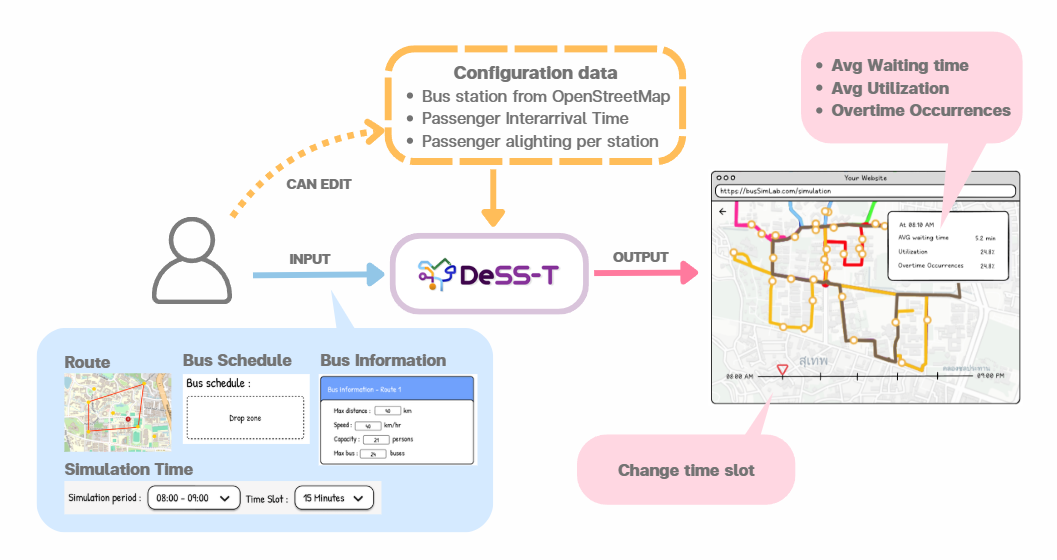
\includegraphics[width=\textwidth,height=0.9\textheight,keepaspectratio]{overview.png}
    \caption{แผนภาพโดยรวมของโครงงาน}
    \label{fig:overview}
\end{figure}

\subsection{Input data (Scenario data)}
\begin{mypara}
  \indent เป็นข้อมูลที่ผู้ใช้สามารถปรับเปลี่ยนพารามิเตอร์ได้บ่อย ๆ เพื่อจำลองสถานการณ์ต่าง ๆ 
  สำหรับการเปรียบเทียบและวางแผน ประกอบด้วย เส้นทางการให้บริการของรถในแต่ละสายบริการ 
  ตารางเวลาการออกรถ ช่วงเวลาที่ต้องการดูผลการจําลอง ข้อมูลของรถซึ่งมี 
  ความจุผู้โดยสารระยะทางที่สามารถวิ่งได้สูงสุด ความเร็วในการวิ่ง
\end{mypara}
\subsection{Configuration data (Base data)}
\begin{mypara}
  \indent เป็นส่วนของข้อมูลที่ใช้เป็นพื้นฐานในการจำลองซึ่งจะไม่ค่อยมีการเปลี่ยนแปลงบ่อย 
  ได้แก่ ข้อมูลช่วงระยะห่างของเวลาที่ผู้โดยสารแต่ละคนมาถึงที่สถานี ข้อมูลของจำนวนผู้โดยสารที่ลงจากรถในแต่ละสถานี 
  และข้อมูลที่เกี่ยวข้องกับสถานีซึ่งจะเก็บในรูปแบบของ network model ซึ่งจะมี 
  node เป็นรายชื่อสถานี และ มี edge เป็นระยะทางละหว่างแต่ละสถานี
  \end{mypara}
\subsection{Simulation Engine}
\begin{mypara}
  \indent เป็นส่วนที่ทำหน้าที่ในการจำลองระบบขนส่งสาธารณะตามข้อมูลที่ได้รับจากส่วน input 
  และ configuration data ซึ่งจะใช้เทคนิคการจำลองแบบเหตุการณ์ไม่ต่อเนื่อง (discrete-event simulation) 
  ในการจำลองระบบขนส่งสาธารณะ 
\end{mypara}
\subsection{Output}
\begin{mypara}
  \indent เป็นส่วนที่แสดงผลลัพธ์ที่ได้จากการจำลอง โดยจะมีข้อมูล การรอเฉลี่ยของผู้โดยสาร อัตราการใช้งานของรถ 
  และอัตราการเกิดเหตุการณ์ที่รถบัสมีการใช้งานเกินเวลาหรือระยะทางที่กำหนด
  ซึ่งจะมีข้อมูลแสดงทั้งข้อมูลรวมทุกสถานี และข้อมูลรายละเอียดของแต่ละสถานีแยกกัน รวมถึงจะมี dashboard 
  สำหรับแสดงผลลัพธ์ในรูปแบบกราฟเพื่อให้ผู้ใช้สามารถวิเคราะห์ข้อมูลได้ง่ายขึ้น
\end{mypara}
\section{ ขั้นตอนการทำงาน (Process Overview)}
\begin{mypara}
    \indent โครงงานนี้ทำงานโดยนำข้อมูลจากผู้ใช้ (input) มาจำลองระบบขนส่งสาธารณะ 
    โดยอ้างอิงจาก configuration data ซึ่งประกอบด้วยข้อมูลหลายประเภท 
    โดยบางส่วนจะถูกนำไปสร้างเป็น distribution function เพื่อใช้ในการสุ่มพฤติกรรมของผู้โดยสาร 
    ขณะที่ข้อมูลอีกส่วนจะถูกนำมาใช้โดยตรง ใน simulation engine ซึ่งจะประมวลผลด้วย
    เทคนิคการจำลองแบบเหตุการณ์ไม่ต่อเนื่อง (discrete-event simulation) 
    เพื่อสร้างผลลัพธ์เชิงสถิติที่สะท้อนประสิทธิภาพของระบบขนส่งสาธารณะมาแสดงผลในส่วน output
\end{mypara}

\section{User Interface (UI)}
\begin{mypara}
    \indent โครงงานนี้มีการออกแบบเพื่อให้ผู้ใช้สามารถป้อนข้อมูลที่จำเป็นสำหรับ
    การจำลองระบบขนส่งสาธารณะได้อย่างสะดวกและไม่ซับซ้อน 
    โดยข้อมูลที่มีการเปลี่ยนแปลงบ่อย จะถูกจัดให้อยู่ในส่วนของ input 
    ซึ่งสามารถเข้าถึงและแก้ไขได้ง่ายโดยไม่ต้องผ่านขั้นตอนที่ซับซ้อน 
    ส่วนข้อมูลพื้นฐานของระบบขนส่งสาธารณะ จะถูกจัดเก็บแยกเป็น configuration data 
    เพื่อให้ง่ายต่อการนำมาใช้ซ้ำ และมี workspace สำหรับการจัดการข้อมูลที่ช่วยให้ผู้ใช้สามารถ 
    clone configuration data หรือ input จากผู้อื่นมาใช้งานและปรับแก้ได้สะดวก

  \indent ในส่วนของ output ได้ออกแบบให้สามารถแสดงผลได้ทั้งมุมมองภาพรวมและ
  รายละเอียดรายสถานี เพื่อให้ผู้ใช้ตรวจสอบข้อมูลเชิงลึกได้อย่างครบถ้วน นอกจากนี้ยังมี 
  dashboard สรุปผล ที่นำเสนอข้อมูลในรูปแบบกราฟและตัวชี้วัดสำคัญ 
  เพื่อช่วยให้ผู้ใช้สามารถเปรียบเทียบและวิเคราะห์ประสิทธิภาพของระบบขนส่งสาธารณะ
  ได้อย่างสะดวกและมีประสิทธิภาพ
\end{mypara}

\subsection{การจัดกลุ่มผู้ใช้ (User Grouping)}
\begin{mypara}
\indent โครงงานนี้มีการจัดกลุ่มผู้ใช้เป็น 2 กลุ่มหลัก ได้แก่
\begin{itemize}
    \item ผู้ใช้ที่ลงทะเบียน (Registered Users): กลุ่มนี้เป็นผู้ใช้ที่สร้างบัญชีและเข้าสู่ระบบเรียบร้อยแล้ว 
    สามารถเข้าถึงฟังก์ชันทั้งหมดของระบบ สามารถบันทึกการจำลองหรือ upload ข้อมูลขึ้นไปบน workspace ได้ 
    \item ผู้ใช้ที่ไม่ได้ลงทะเบียน (Guest Users / Unregistered Users): กลุ่มนี้เป็นผู้ใช้ทั่วไปที่ไม่ได้สร้างบัญชี 
    สามารถใช้ระบบจำลองได้แบบจำกัดฟังก์ชัน โดยทำการจำลองและดูผลลัพธ์ได้ชั่วคราว 
    แต่ไม่สามารถบันทึกข้อมูลได้
\end{itemize}
\end{mypara}
\section{User Flow}

\begin{mypara}

\begin{itemize}
    \item ผู้ใช้ที่ไม่ได้ลงทะเบียน (Guest Users / Unregistered Users)
    \begin{figure}[H]
    \centering
    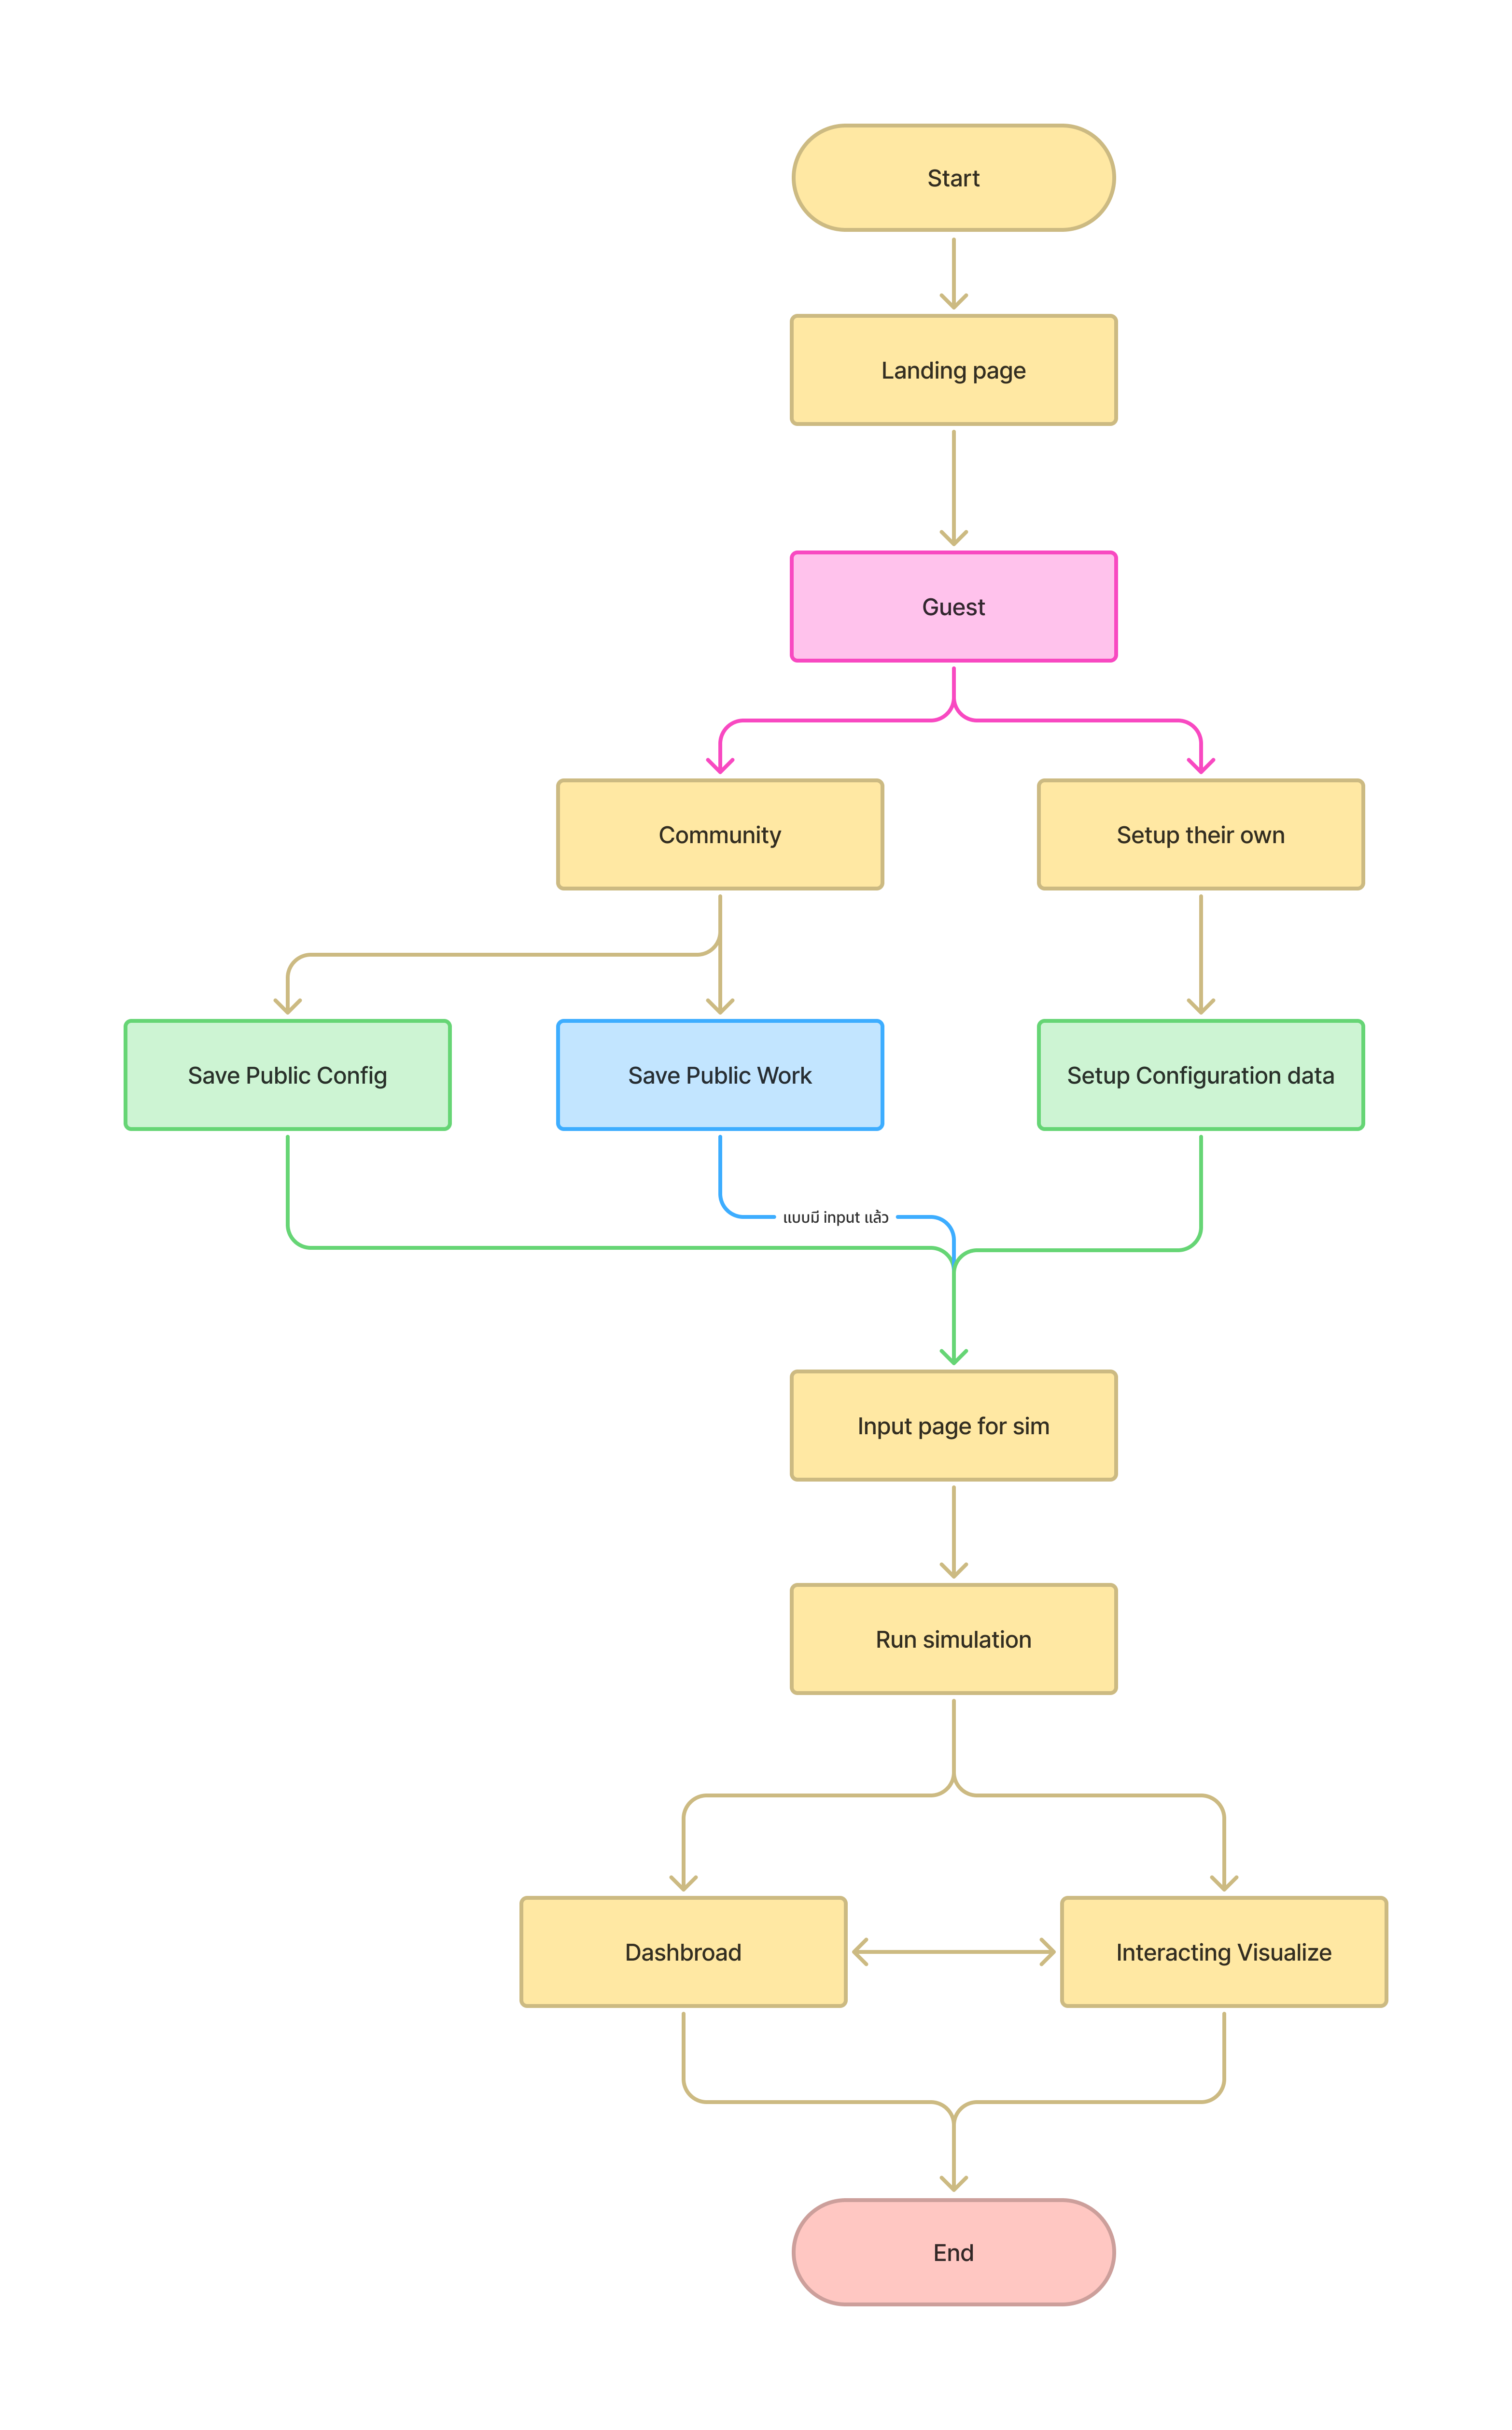
\includegraphics[width=\textwidth,height=0.6\textheight,keepaspectratio]{User_flow_-_guest.png}
    \caption{User flow  ของผู้ใช้ที่ไม่ได้ลงทะเบียน}
    \label{fig:UserFlowUnregistered}
    \end{figure}
    \newpage
    \item ผู้ใช้ที่ลงทะเบียน (Registered Users)
    \begin{figure}[H]
    \centering
    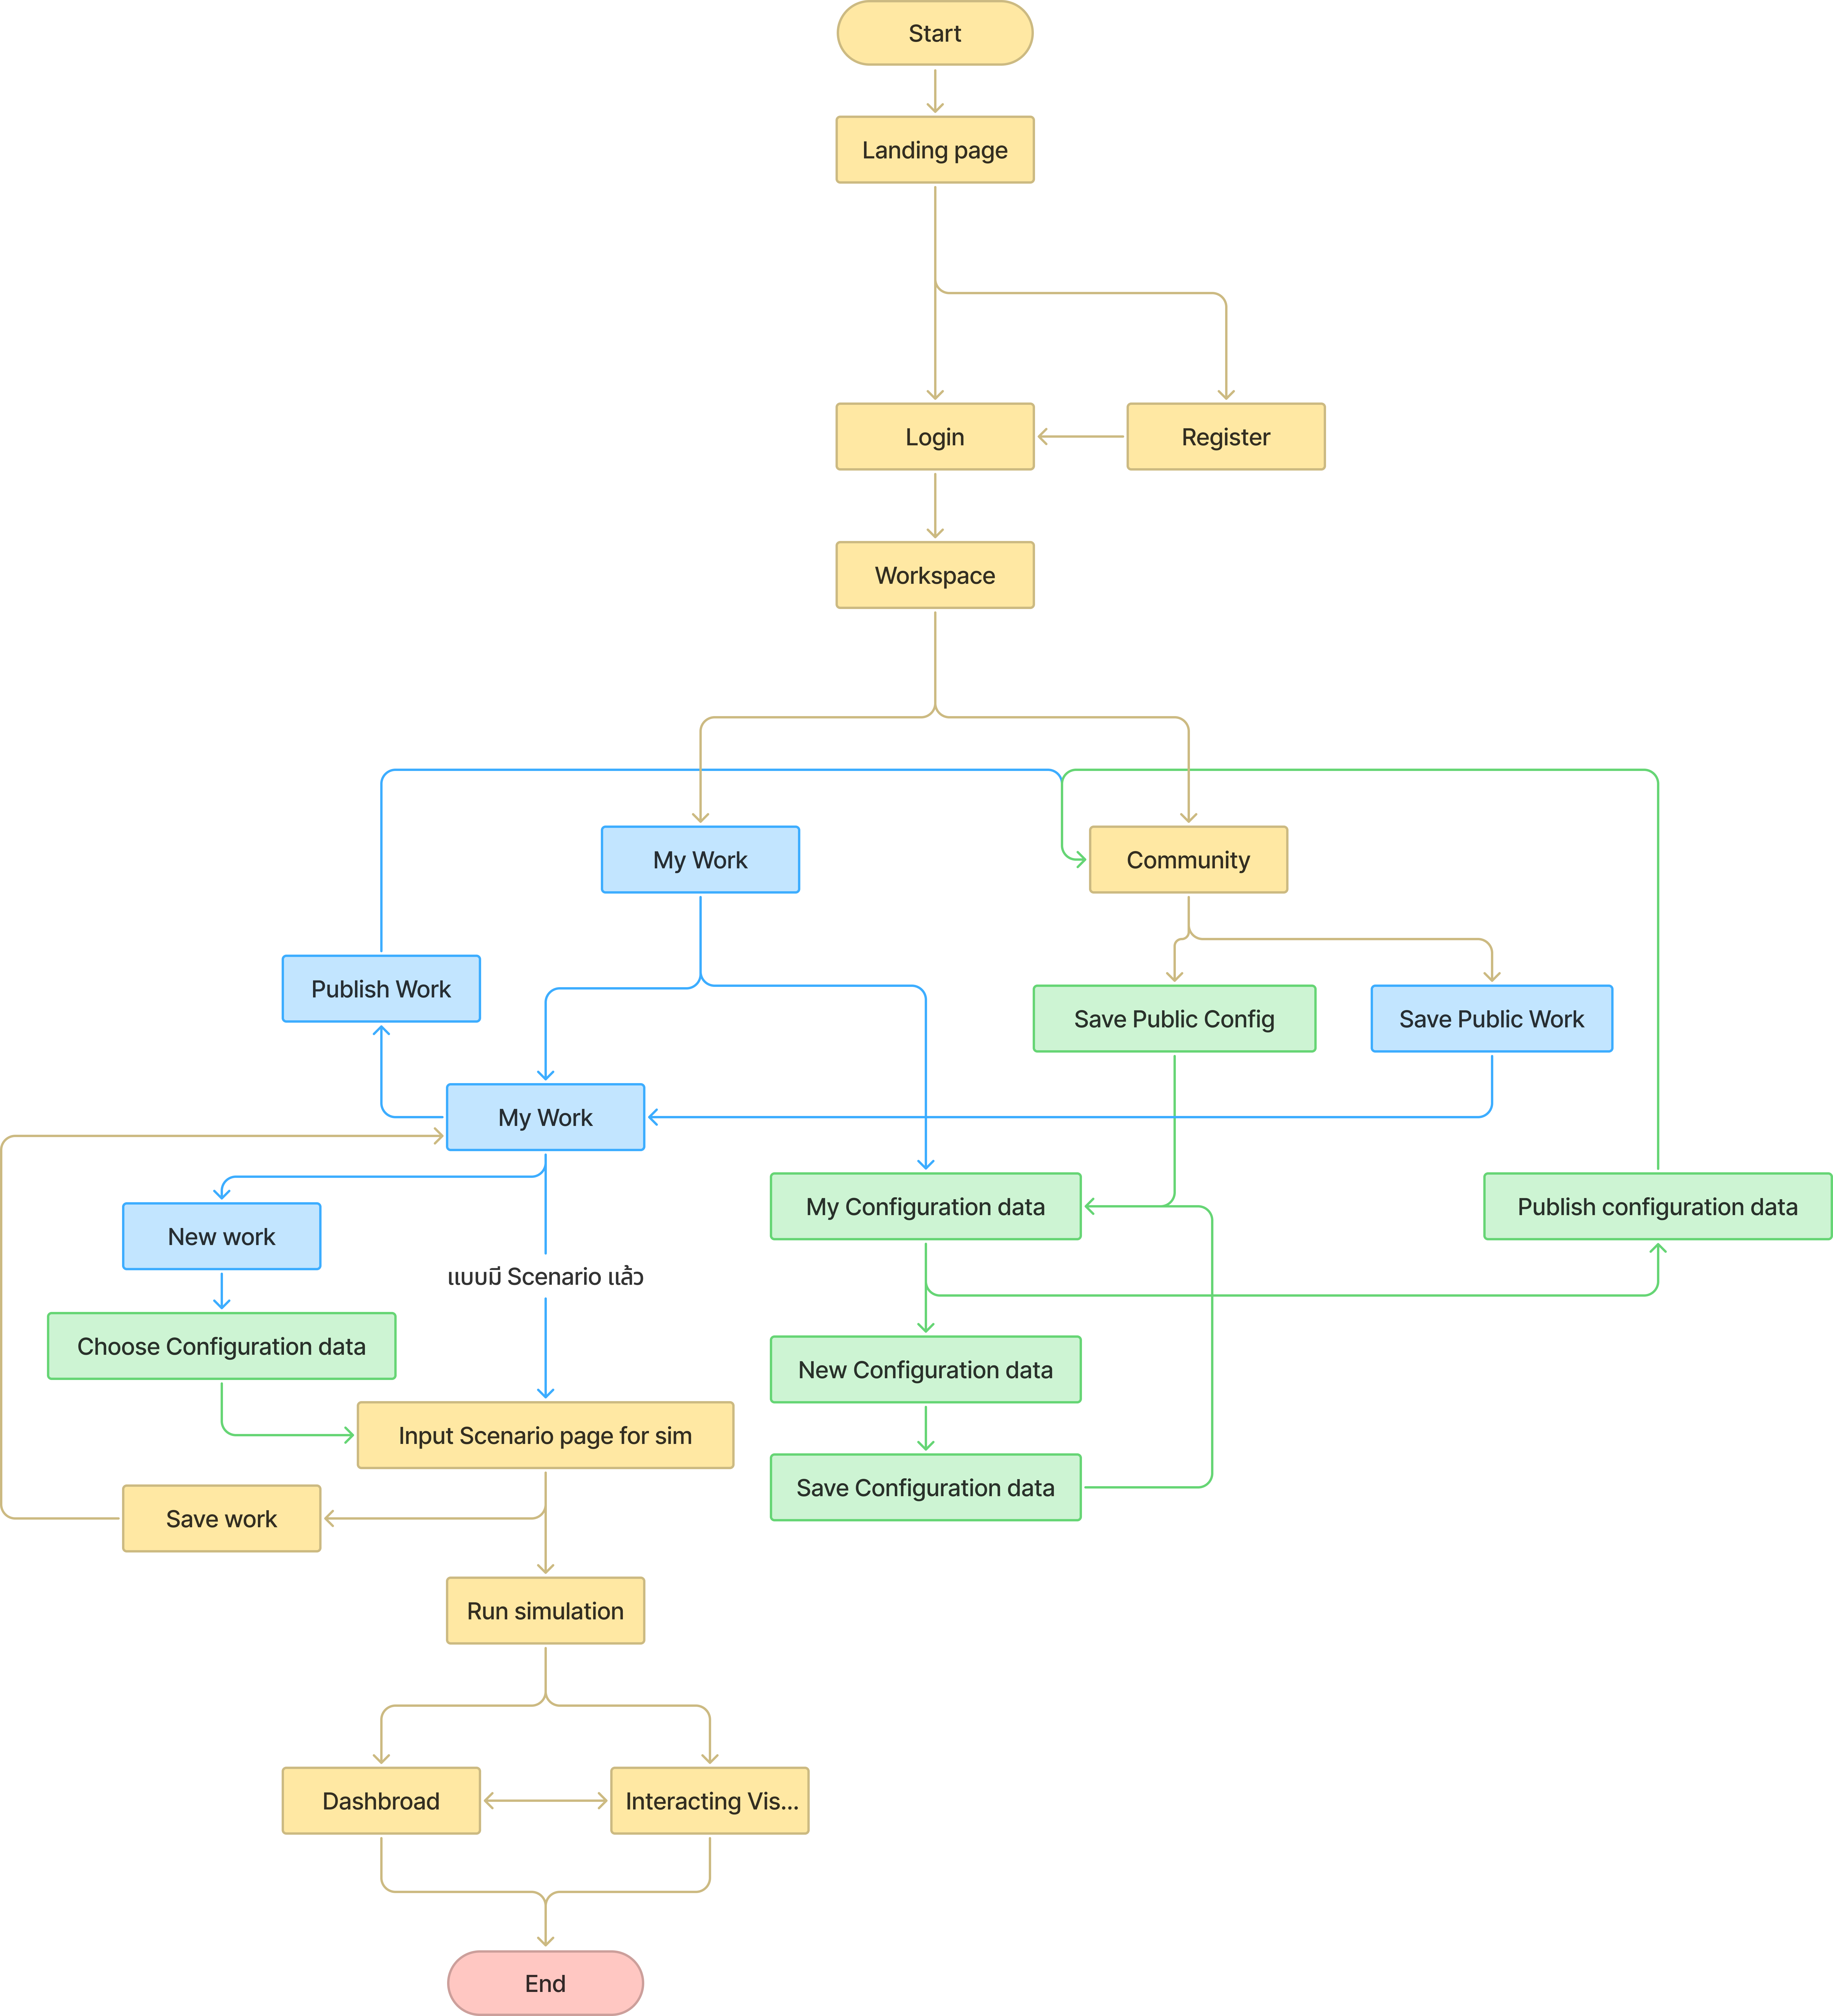
\includegraphics[width=\textwidth,height=0.9\textheight,keepaspectratio]{User_flow_-_login.png}
    \caption{User flow ของผู้ใช้ที่ลงทะเบียน}
    \label{fig:UserFlowRegistered}
    \end{figure}
    

\end{itemize}
\end{mypara}
\newpage
\section{Wireframe}
\begin{mypara}
    \indent โครงงานนี้มีการออกแบบ Wireframe สำหรับหน้าต่างๆ ของระบบ 
    เพื่อใช้เป็นแนวทางในการพัฒนาและทดสอบระบบ โดย Wireframe ที่ออกแบบมีดังนี้

\subsection{Wireframe ผู้ใช้ที่ไม่ได้ลงทะเบียน (Guest Users / Unregistered Users)}
\begin{itemize}
    \item Step 1: ผู้ใช้จะเข้าสู่หน้า Landing page เพื่อเลือกระหว่างจะเข้าใช้ในโหมด Guest user หรือ Login user
      \begin{figure}[H]
        \centering
        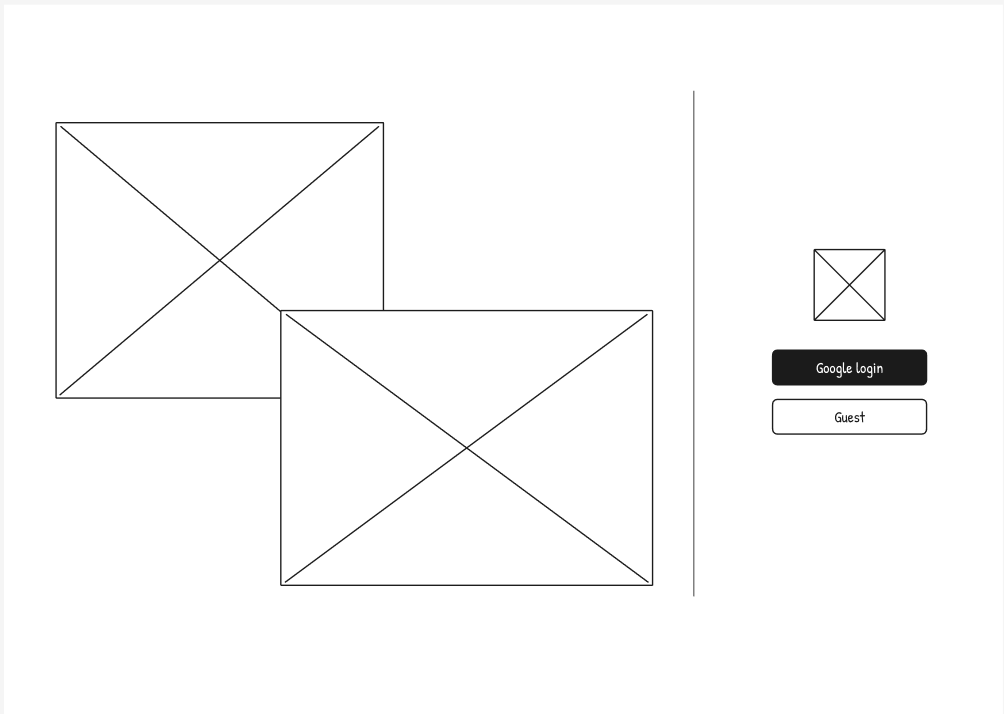
\includegraphics[scale=0.35]
        {homepage.png}
        \caption{Wireframe ของหน้า Landing page}
        \label{fig:WireframeHomepage}
      \end{figure}

    \item Step 2: Guest user สามารถเลือกว่าจะใช้ข้อมูลที่มีอยู่ใน Community หรือเลือกที่จะ Setup ข้อมูลทั้งหมดเอง
      \begin{figure}[H]
        \centering
        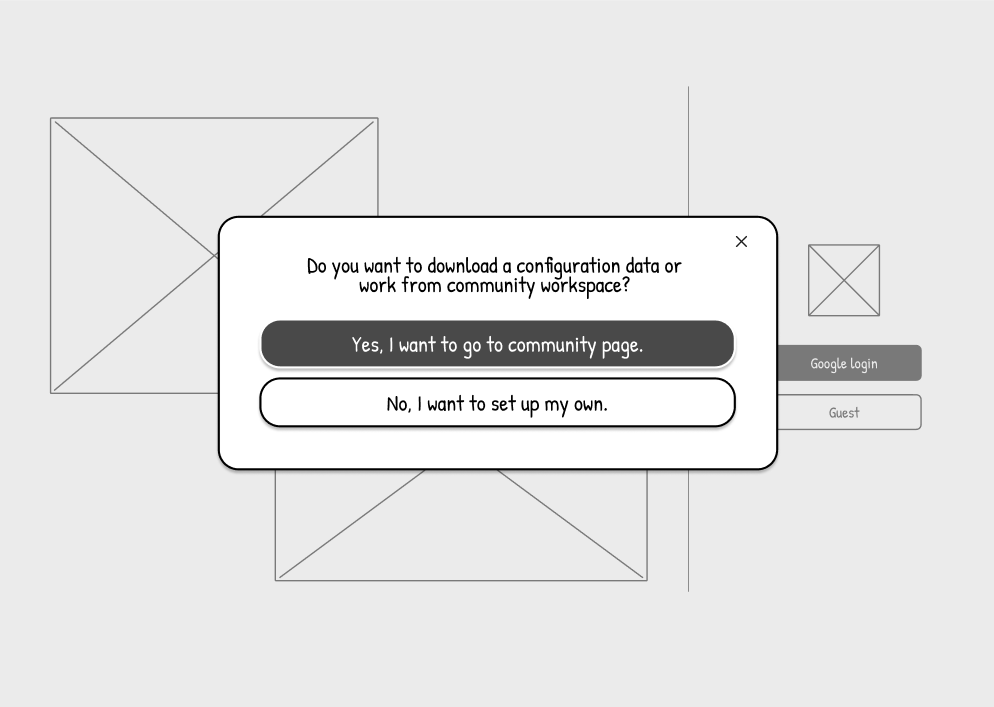
\includegraphics[scale=0.35]
        {guest_login.png}
        \caption{Wireframe ของหน้า Guest Decision}
        \label{fig:WireframeGuestDecision}
      \end{figure}

    \item Step 3: การใช้ข้อมูล Configuration data
    \begin{itemize}
        \item กรณีที่เลือกใช้จากข้อมูลที่มีอยู่ใน Community
          \begin{figure}[H]
            \centering
            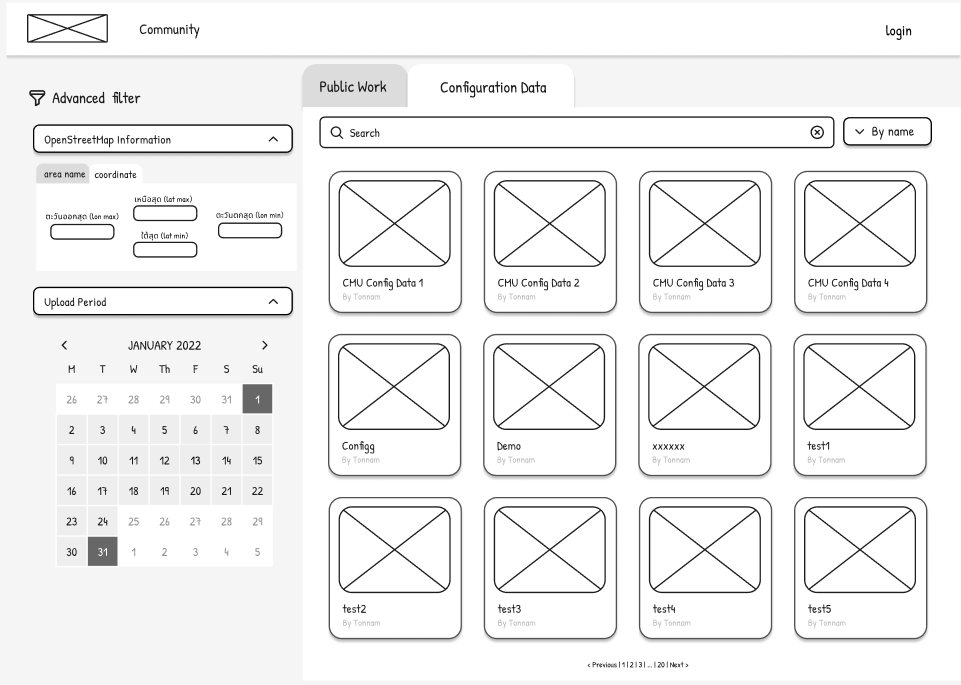
\includegraphics[scale=0.4]{conf_commu_guest.png}
            \caption{Wireframe ของหน้า Community Configuration data}
            \label{fig:WireframeCommunityConfigGuest}
          \end{figure}

          \begin{figure}[H]
            \centering
            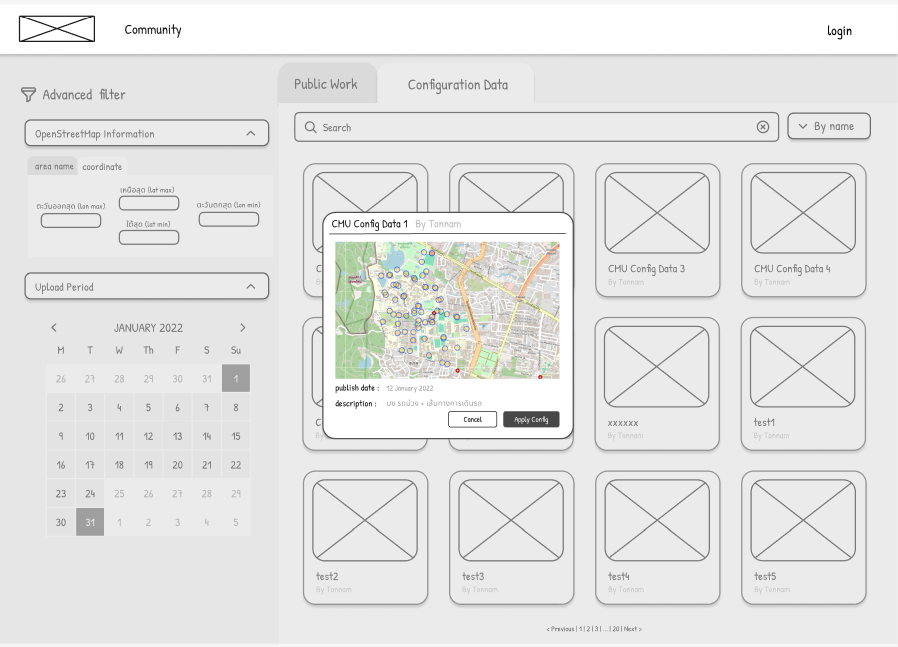
\includegraphics[scale=0.4]{conf_commu_detail_guest.png}
            \caption{Wireframe ของหน้ารายละเอียด Configuration data ใน Community}
            \label{fig:WireframeCommunityConfigDetailGuest}
          \end{figure}

        \newpage
        \item กรณีที่ผู้ใช้เลือก Setup ข้อมูลทั้งหมดเอง จะเข้าสู่การ Setup Configuration ด้วยตนเอง
          \begin{figure}[H]
            \centering
            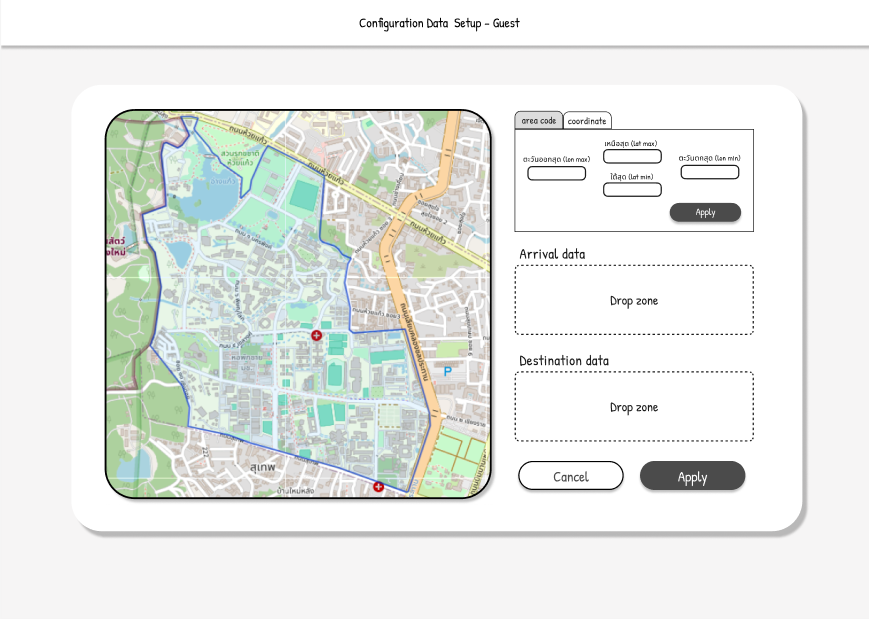
\includegraphics[scale=0.4]{conf_setup_guest.png}
            \caption{Wireframe ของหน้า Setup Configuration data สำหรับ Guest}
            \label{fig:WireframeSetupConfigGuest}
          \end{figure}
    \end{itemize}

    \item Step 4: หลังจาก Setup Configuration data ทั้งหมดเรียบร้อยจะเข้าสู่หน้า Input page เพื่อกรอกข้อมูลสำหรับการจำลองบน Scenario ต่างๆ
      \begin{figure}[H]
        \centering
        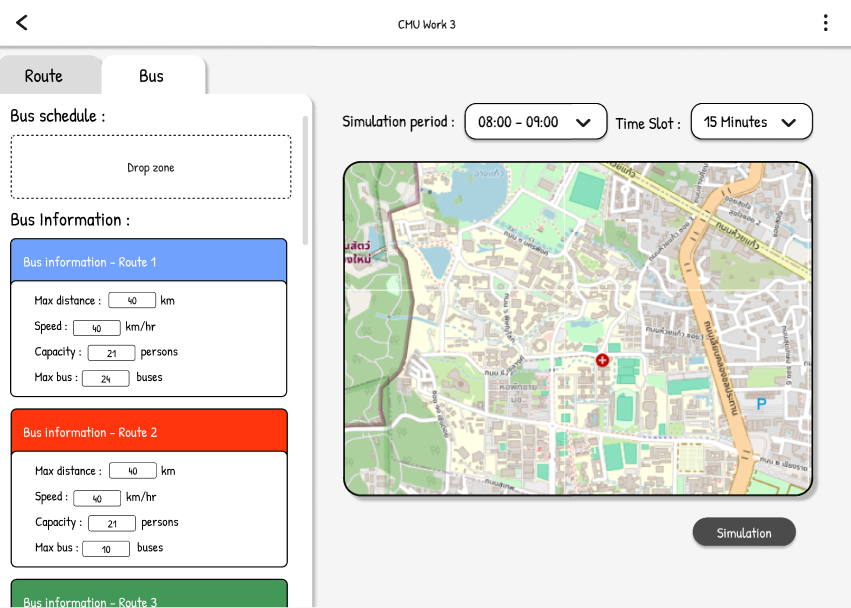
\includegraphics[scale=0.4]{input_bus.png}
        \caption{Wireframe ของหน้า Input page (bus) }
        \label{fig:WireframeInputGuest}
      \end{figure}
      \begin{figure}[H]
        \centering
        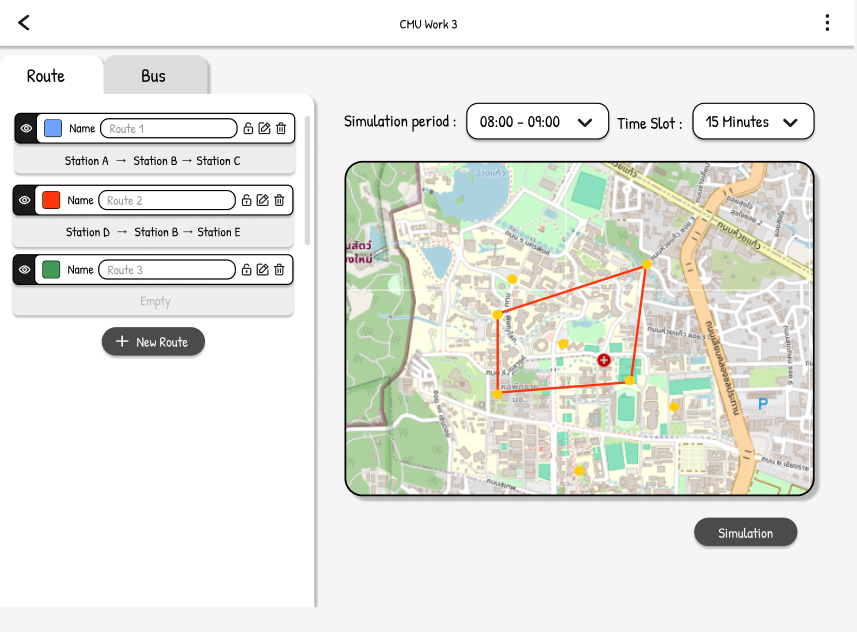
\includegraphics[scale=0.4]{input_route.png}
        \caption{Wireframe ของหน้า Input page (route) }
        \label{fig:WireframeInputRouteGuest}
      \end{figure}

    \item Step 5: หลังจากผู้ใช้กดปุ่ม Run simulation แล้ว User จะสามารถเลือกดู  Dashboard สรุปผลข้อมูล 
    หรือ Interacting Visualize
      \begin{figure}[H]
        \centering
        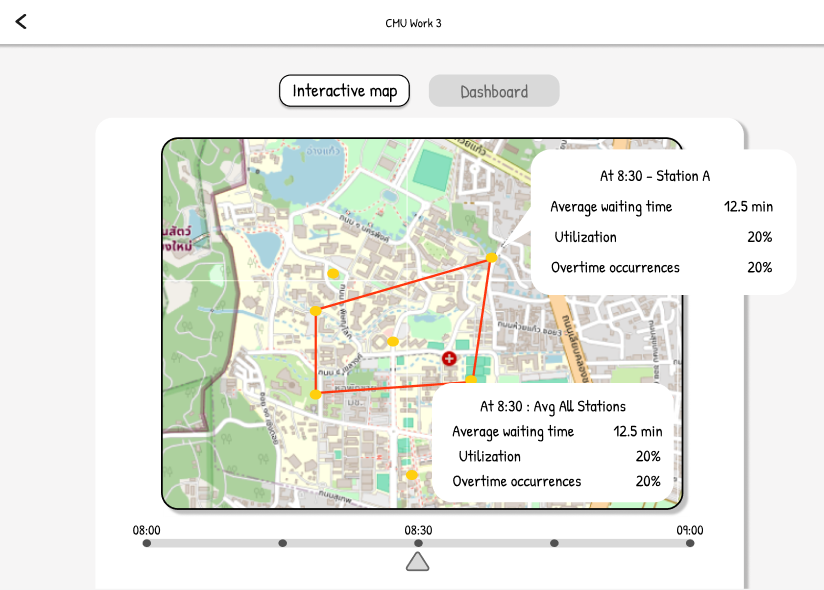
\includegraphics[scale=0.4]{output_show.png}
        \caption{Wireframe ของหน้าแสดงผลลัพธ์หลังจาก Run Simulation}
        \label{fig:WireframeOutputGuest}
      \end{figure} 

      \begin{figure}[H]
        \centering
        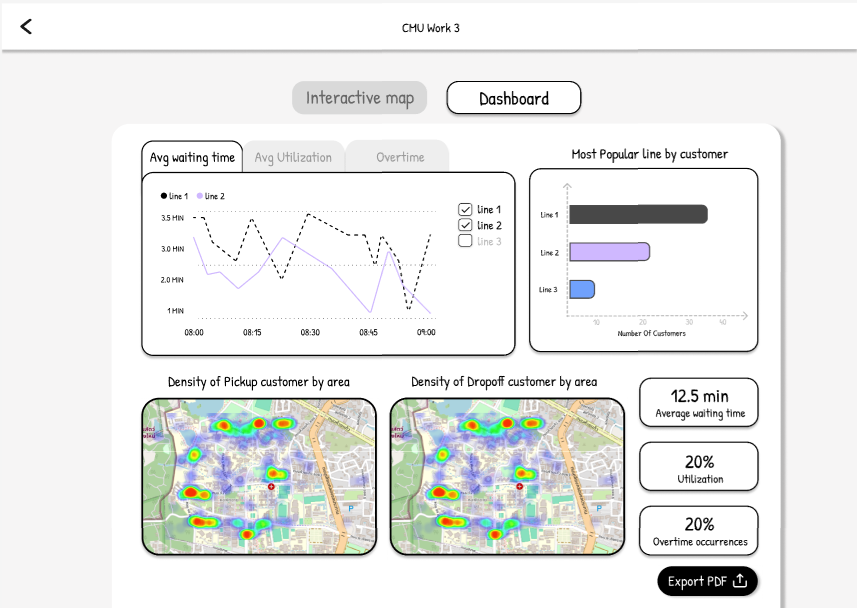
\includegraphics[scale=0.4]{dashboard.png}
        \caption{Wireframe ของหน้า Dashboard }
        \label{fig:WireframeDashboardGuest}
      \end{figure}
    
\end{itemize} 


\subsection{Wireframe ของผู้ใช้ที่ลงทะเบียน (Registered Users)}
\begin{itemize}
    \item Step 1:  ผู้ใช้จะเข้าสู่หน้า Landing page เพื่อเลือกระหว่างจะเข้าใช้ในโหมด Guest user หรือ Login user
    \begin{figure}[H]
    \centering
    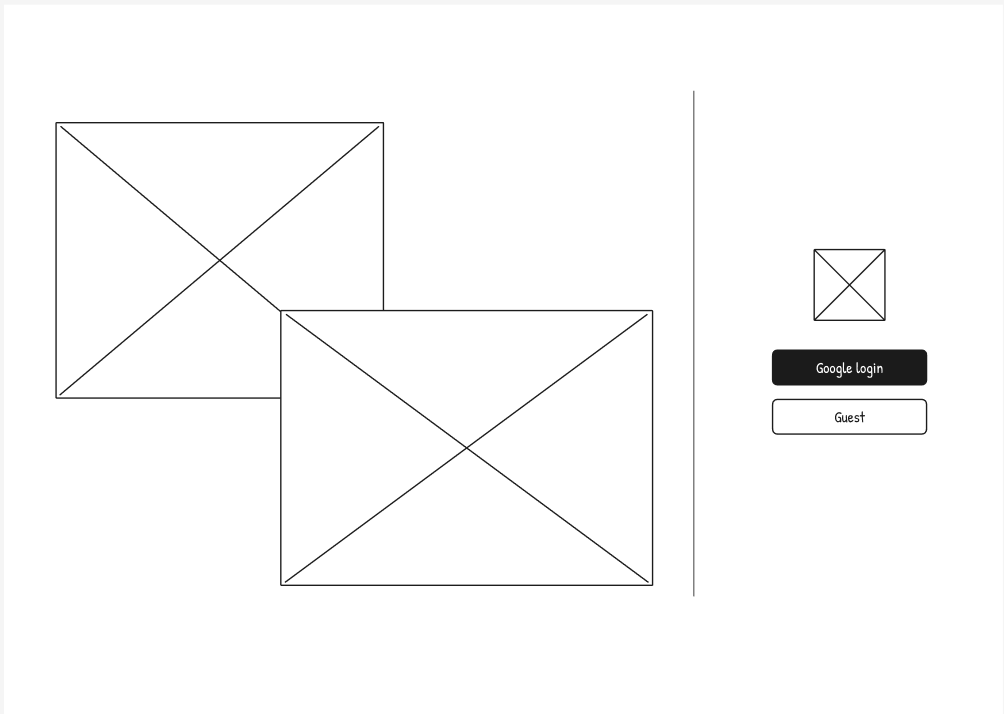
\includegraphics[scale=0.4]
    {homepage.png}
    \caption{Wireframe ของหน้า Landing page}
    \label{fig:WireframeHomepageLogin}
    \end{figure}

    \newpage
    \item Step 2: หลังจากเข้าสู่ระบบผู้ใช้จะเข้าสู่หน้า My work ซึ่งเป็นการจัดการงานทั้งหมดของผู้ใช้
    \begin{itemize}
      \item ในหน้า My work ผู้ใช้สามารถเลือกใช้งานหรือ Publish งาน
        \begin{figure}[H]
          \centering
          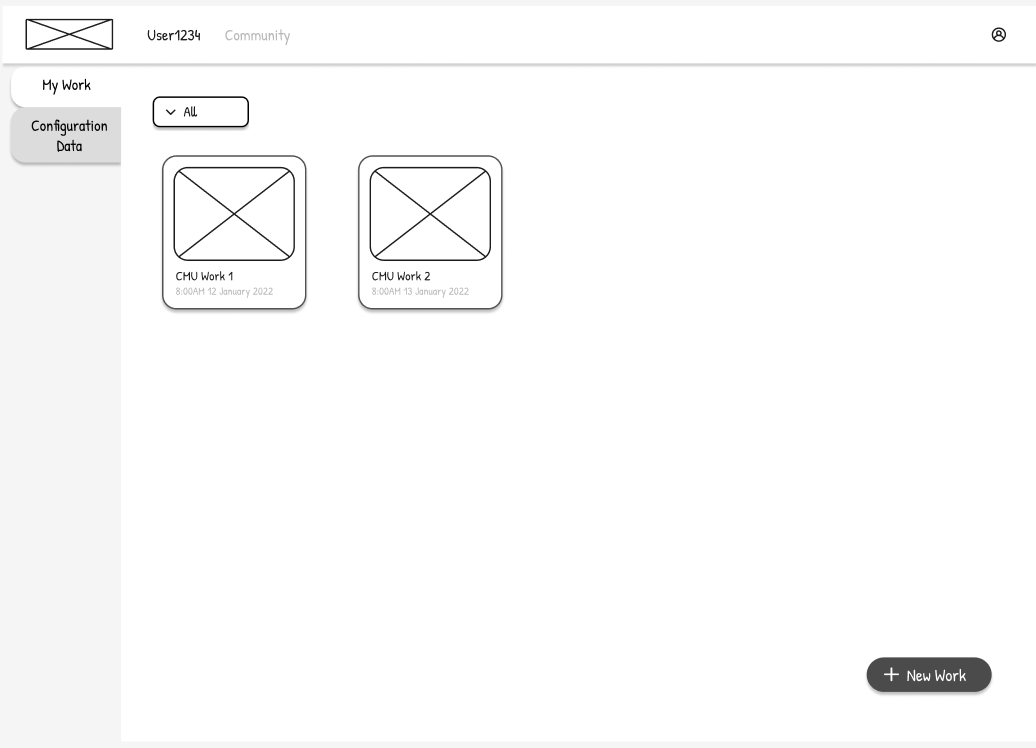
\includegraphics[scale=0.4]{my_work.png} 
          \caption{Wireframe ของหน้า My work}
          \label{fig:WireframeMyWork}
        \end{figure}

        \begin{figure}[H]
          \centering
          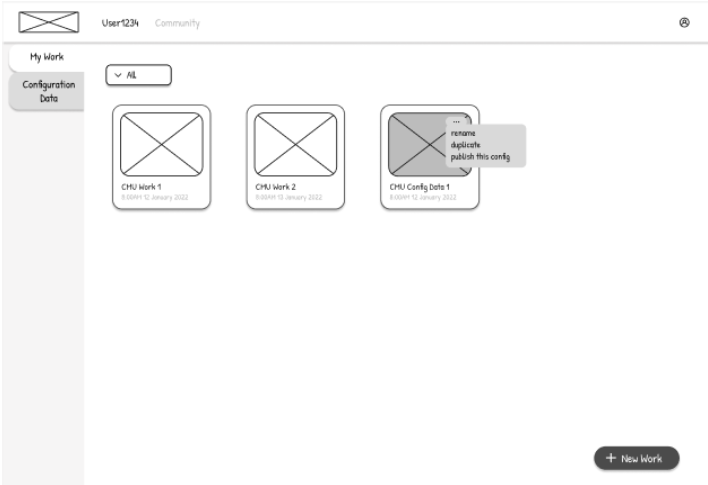
\includegraphics[scale=0.6]{my_work_publish.png} 
          \caption{Wireframe ของหน้า My work ในกรณีที่ Publish งาน}
          \label{fig:WireframeMyWorkPublish}
        \end{figure}
        
      \newpage
      \item  ผู้ใช้สามารถสร้าง Work ใหม่ได้ด้วยการกดที่ปุ่ม New work โดยการสร้าง Work จะต้องอ้างอิงกับ Configuration data ที่มีอยู่
        \begin{figure}[H]
        \centering
        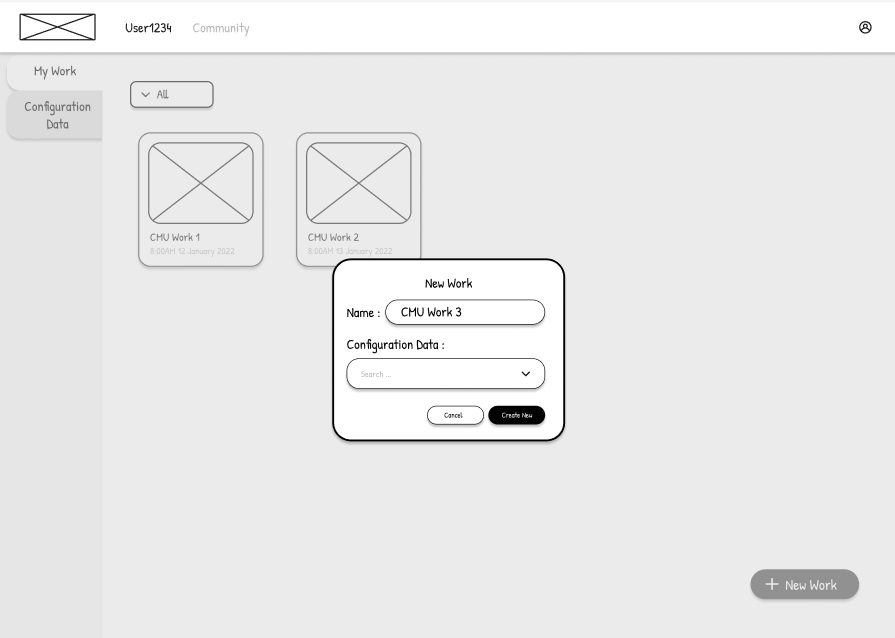
\includegraphics[scale=0.4]{new_work.png}
        \caption{Wireframe ของหน้า New work}
        \label{fig:WireframeNewWork}
        \end{figure}
    \end{itemize}

    \item Step 3: การใช้ข้อมูล Configuration data
    \begin{itemize}
        \item กรณีที่เลือกใช้จากข้อมูลที่มีอยู่ใน Community
          \begin{figure}[H]
            \centering
            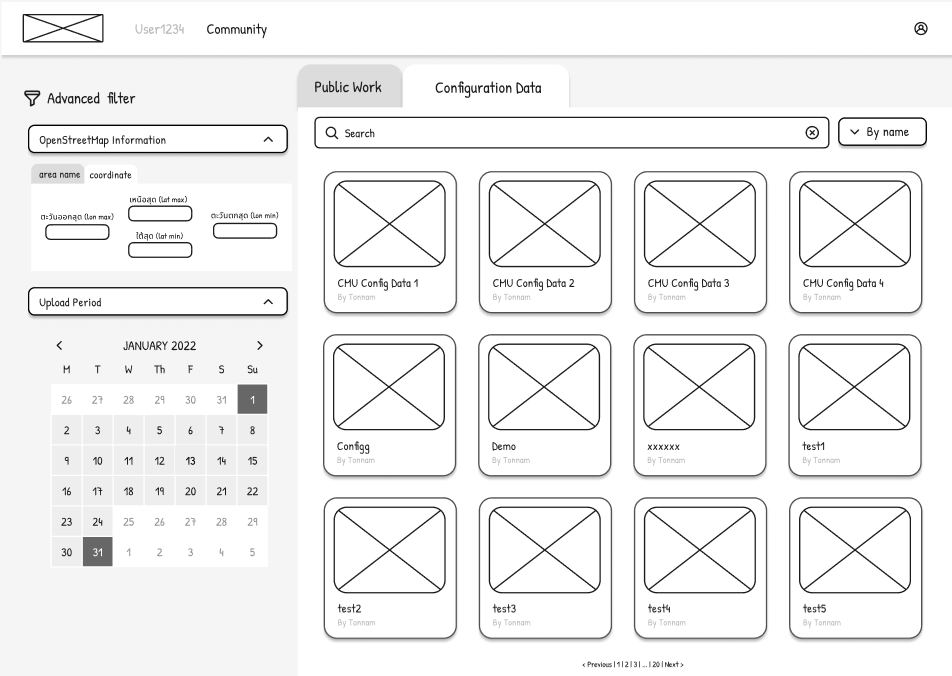
\includegraphics[scale=0.4]{conf_commu.png}
            \caption{Wireframe ของหน้า Community Configuration data}
            \label{fig:WireframeCommunityConfigLogin}
          \end{figure}

          \begin{figure}[H]
            \centering
            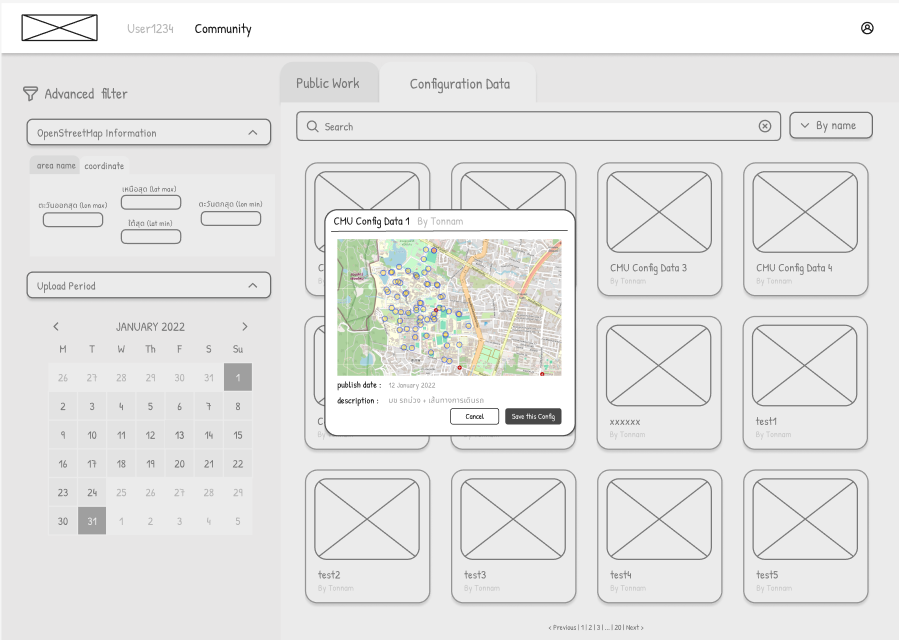
\includegraphics[scale=0.4]{conf_commu_detail_reg.png}
            \caption{Wireframe ของหน้ารายละเอียด Configuration data ใน Community}
            \label{fig:WireframeCommunityConfigDetailLogin}
          \end{figure}

        \item ผู้ใช้สามารถสร้าง Configuration data ใหม่ได้ด้วยการกดที่ปุ่ม New Configuration และสามารถ Save Configuration เพื่อใช้ในงานต่อไปได้
          \begin{figure}[H]
            \centering
            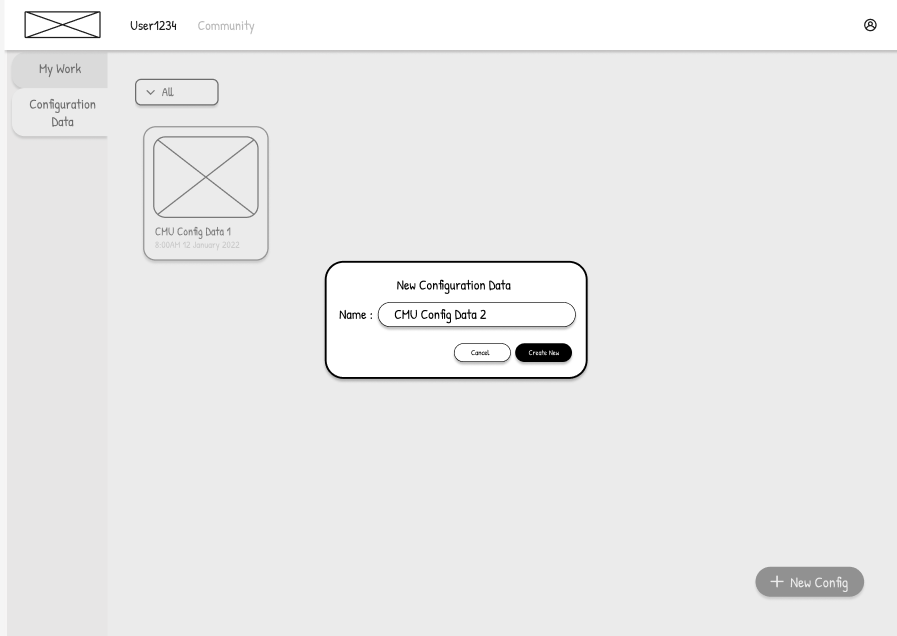
\includegraphics[scale=0.4]{new_conf.png}
            \caption{Wireframe ของหน้า New Configuration data}
            \label{fig:WireframeNewConfigLogin}
          \end{figure}

          \begin{figure}[H]
            \centering
            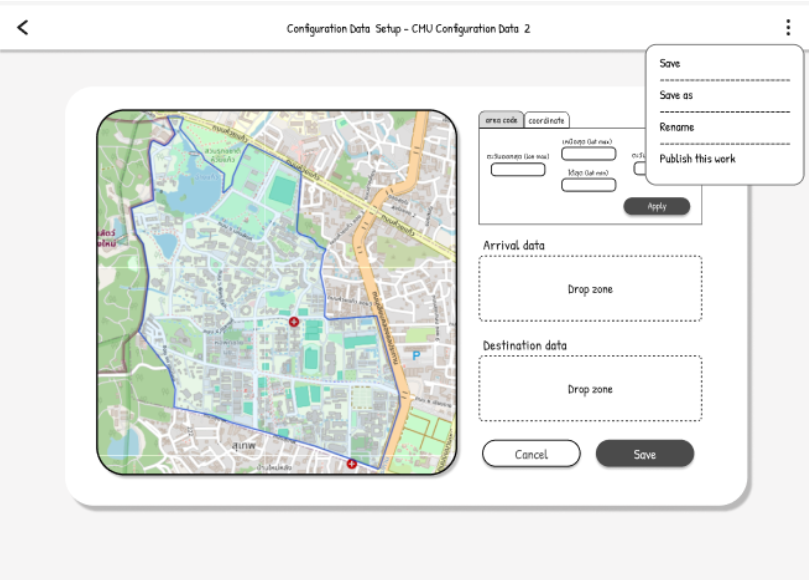
\includegraphics[scale=0.4]{conf_setup_reg.png}
            \caption{Wireframe ของหน้า Setup Configuration data สำหรับผู้ใช้ที่ลงทะเบียน}
            \label{fig:WireframeSetupConfigLogin}
          \end{figure}

    \end{itemize}

    \item Step 4: หน้า Input page เพื่อกรอกข้อมูลสำหรับการจำลองบน Scenario ต่างๆ
      \begin{figure}[H]
        \centering 
        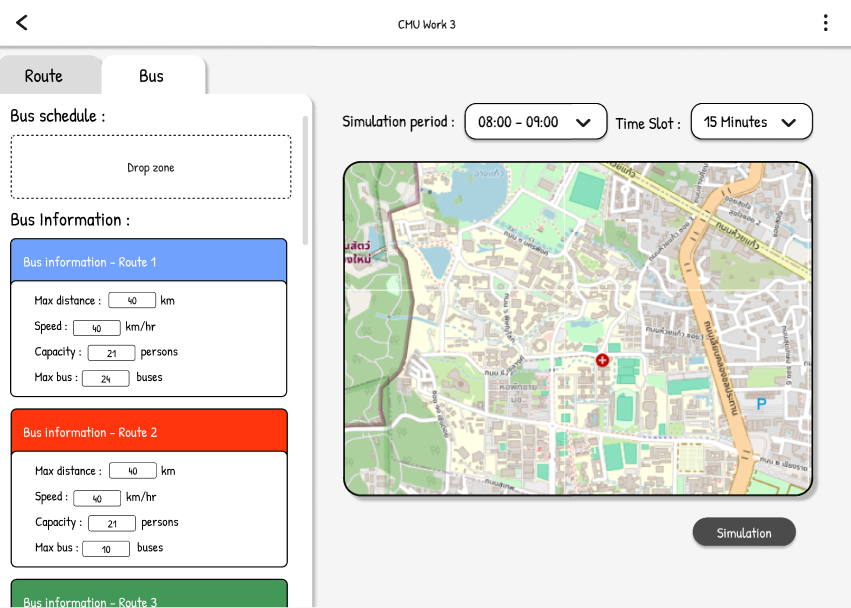
\includegraphics[scale=0.4]{input_bus.png}
        \caption{Wireframe ของหน้า Input page (bus) }
        \label{fig:WireframeInputLogin}
      \end{figure}

      \begin{figure}[H]
        \centering
        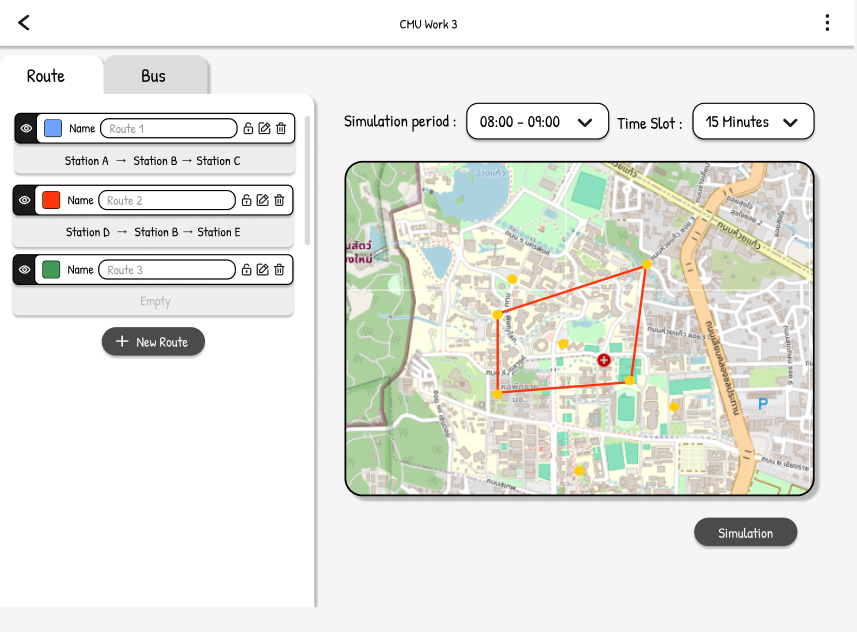
\includegraphics[scale=0.4]{input_route.png}
        \caption{Wireframe ของหน้า Input page (route) }
        \label{fig:WireframeInputRouteLogin}
      \end{figure}

    \item Step 5: หลังจากผู้ใช้กดปุ่ม Run simulation แล้ว User จะสามารถเลือกดู  Dashboard สรุปผลข้อมูล 
      \begin{figure}[H]
        \centering
        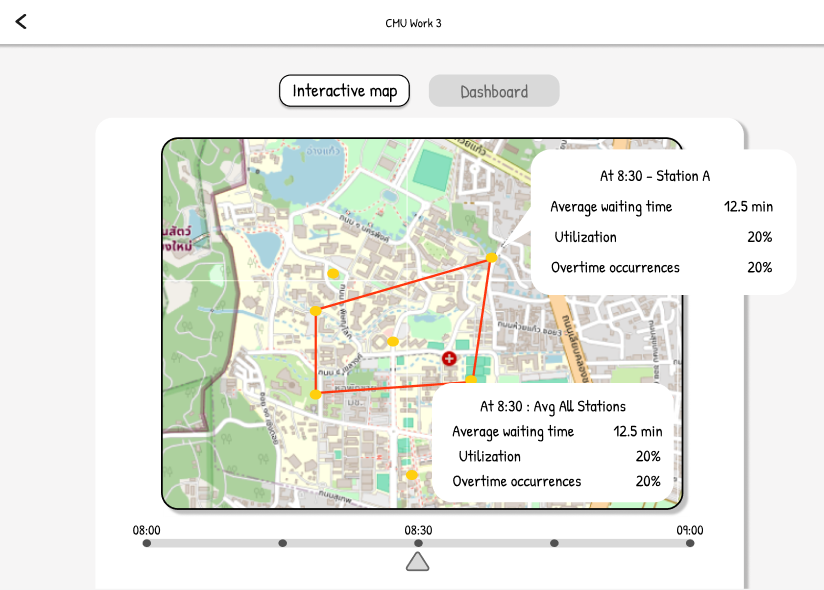
\includegraphics[scale=0.4]{output_show.png}
        \caption{Wireframe ของหน้าแสดงผลลัพธ์หลังจาก Run simulation}
        \label{fig:WireframeOutputLogin}
      \end{figure}

      \begin{figure}[H]
        \centering
        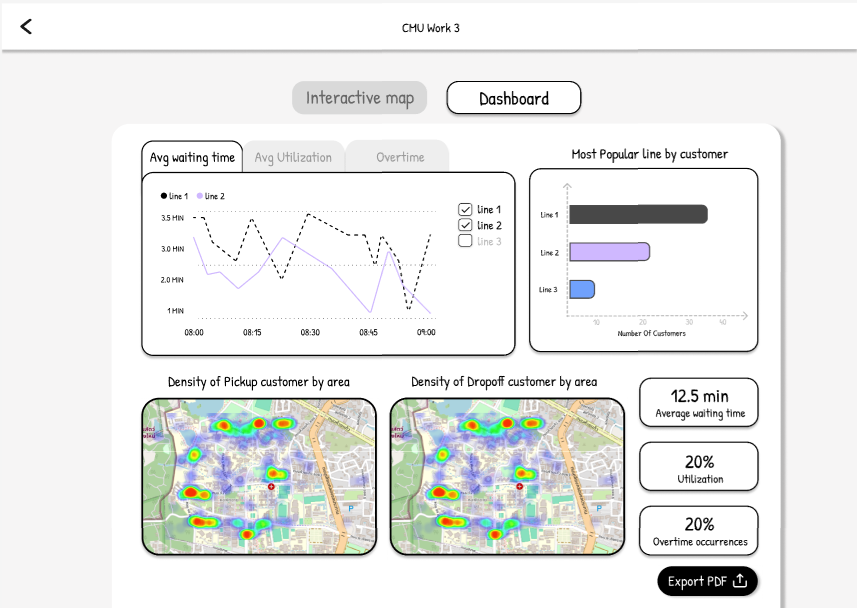
\includegraphics[scale=0.4]{dashboard.png}
        \caption{Wireframe ของหน้า Dashboard }
        \label{fig:WireframeDashboardLogin}
      \end{figure}
    \end{itemize}

\end{mypara}

\section{รูปแบบไฟล์ข้อมูลนำเข้า (Supported Input File Formats)}
  \subsection{รูปแบบไฟล์ช่วงเวลาในการมาถึงของผู้โดยสาร (Passenger Arrival Time File Format)}
  \begin{mypara}
      \indent รูปแบบไฟล์ช่วงเวลาในการมาถึงของผู้โดยสาร ใช้สำหรับเก็บข้อมูลช่วงเวลาที่ผู้โดยสารแต่ละคนมาถึงที่สถานี
      โดยข้อมูลจะถูกจัดเก็บในไฟล์ Excel โดยมีสกุลไฟล์ \texttt{.xlsx} 
      ซึ่งมีโครงสร้างดังแสดงในภาพด้านล่าง
      \begin{figure}[H]
        \centering
        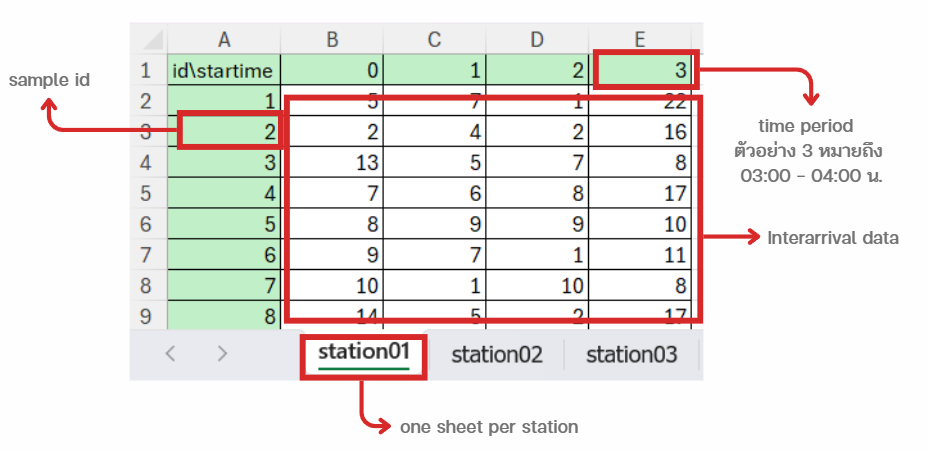
\includegraphics[scale=0.5]{Passenger_Interarrival.png}
        \caption{รูปแบบไฟล์ช่วงเวลาในการมาถึงของผู้โดยสาร}
        \label{fig:PassengerArrivalFileFormat}
      \end{figure}
  \end{mypara}

  \newpage
  \subsection{รูปแบบไฟล์จำนวนผู้โดยสารที่ลงจากรถ (Passenger Alight File Format)}
  \begin{mypara}
      \indent รูปแบบไฟล์จำนวนผู้โดยสารที่ลงจากรถ ใช้สำหรับเก็บข้อมูลจำนวนผู้โดยสารที่ลงจากรถในแต่ละสถานี
      โดยข้อมูลจะถูกจัดเก็บในไฟล์ Excel โดยมีสกุลไฟล์ \texttt{.xlsx} 
      ซึ่งมีโครงสร้างดังแสดงในภาพด้านล่าง
      \begin{figure}[H]
        \centering
        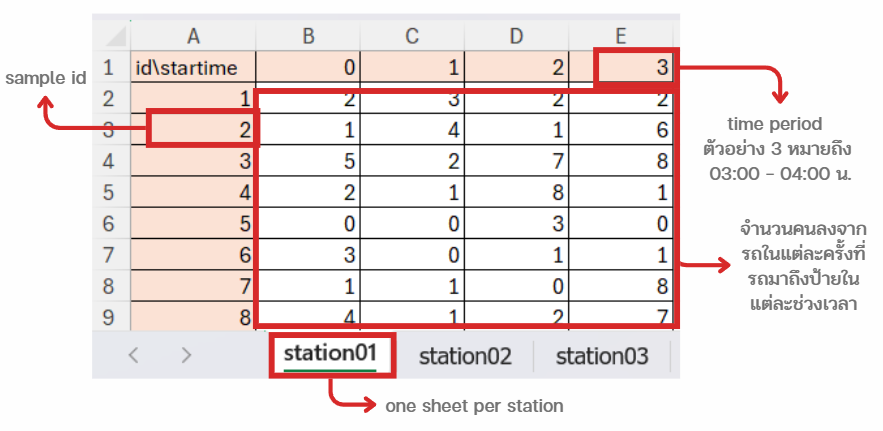
\includegraphics[scale=0.5]{Passenger_alighting.png}
        \caption{รูปแบบไฟล์จำนวนผู้โดยสารที่ลงจากรถ}
        \label{fig:PassengerAlightFileFormat}
      \end{figure}
  \end{mypara}

  \subsection{รูปแบบไฟล์ตารางการเดินรถ (Bus Schedule File Format)}
  \begin{mypara}
      \indent รูปแบบไฟล์ตารางการเดินรถ ใช้สำหรับเก็บข้อมูลเวลาการออกรถของแต่ละสายบริการ 
      โดยข้อมูลจะถูกจัดเก็บในไฟล์ Excel โดยมีสกุลไฟล์ \texttt{.xlsx} 
      ซึ่งมีโครงสร้างดังแสดงในภาพด้านล่าง
      \begin{figure}[H]
        \centering
        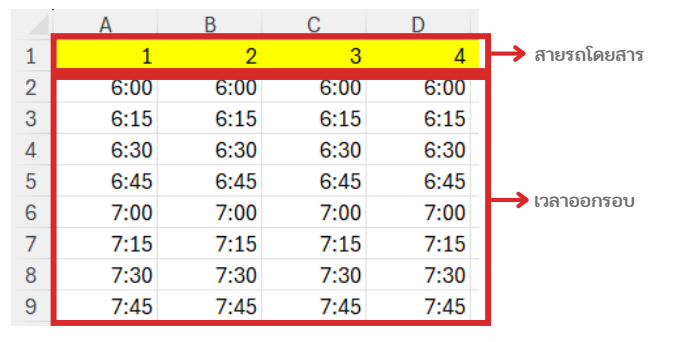
\includegraphics[scale=0.5]{bus_schedule.png}
        \caption{รูปแบบไฟล์ตารางการเดินรถ}
        \label{fig:BusScheduleFileFormat}
      \end{figure}
  \end{mypara}
\chapter{\ifproject%
\ifenglish Experimentation and Results\else การทดลองและผลลัพธ์\fi
\else%
\ifenglish System Evaluation\else การประเมินระบบ\fi
\fi}
\begin{mypara}
    \indent บทนี้จะกล่าวถึงการประเมินระบบทั้งในด้านการทำงานของระบบ ความถูกต้องและความแม่นยำของระบบจำลอง 
    รวมถึงการประเมินจากผู้ใช้งานจริง เพื่อยืนยันความเหมาะสมและประสิทธิภาพของการนำระบบไปประยุกต์ใช้ในสถานการณ์จริง
    โดยมีรายละเอียดการประเมินดังนี้
\end{mypara}

\section{การวัดและประเมินการทำงานของระบบจำลอง}
\begin{itemize}
  \item ความถูกต้องในการสร้าง Configuration data
  
  \item ข้อสอง
  \item ข้อสาม
\end{itemize}
\section{การวัดและประเมินความถูกต้องและความแม่นยำของระบบจำลอง}
\section{การวัดและประเมินด้านการใช้งานจากผู้ใช้จริง}
\ifproject
\include{chapters/conclusion}
\fi

\bibliography{sampleReport}

\ifproject
\normalspacing% ...เนื้อหาทั้งหมด...


\appendix
\include{chapters/appendix}

%% Display glossary (optional) -- need glossary option.
\ifglossary\glossarypage\fi

%% Display index (optional) -- need idx option.
\ifindex\indexpage\fi

\begin{biosketch}
\begin{center}
  \includegraphics[width=1.5in]{mugshot.jpg}
\end{center}
Your biosketch goes here. Make sure it sits inside
the \texttt{biosketch} environment.
\end{biosketch}
\fi % \ifproject



\sloppy
\begin{thebibliography}{99}
    \bibitem{ragsdale2008} Ragsdale, C. T. (2008). 
        \textit{Spreadsheet Modeling \& Decision Analysis: A Practical Introduction to Business Analytics} 
        (6th ed., Chapter~13: Queuing Theory). Cengage Learning.
    \bibitem{kelton2010} Kelton, W. D., Sadowski, R. P., \& Sadowski, D. A. (2010). 
        \textit{Simulation with Arena} (2nd ed.). McGraw-Hill Education (Asia) / McGraw-Hill.
    \bibitem{ref3} Sasibhushana Matcha, et al. (2025). 
        RESTful API Design and Implementation: Best Practices for Building Scalable and Maintainable Web Services. 
        ResearchGate. \url{https://www.researchgate.net/publication/388950588_RESTful_API_Design_and_Implementation_Best_Practices_for_Building_Scalable_and_Maintainable_Web_Services}
    \bibitem{babulak2008} Babulak, E., \& Wang, M. (2008). Discrete event simulation: State of the art. \textit{International Journal of Online Engineering (iJOE)}, 4(1), 60–63. \url{https://doi.org/10.5772/9894}
    \bibitem{rich2023} Rich, J. (2023). Fixed routing or demand-responsive? Agent-based modeling of autonomous vehicle services for first and last mile connections. \textit{Transportation Research Part C: Emerging Technologies}, 145, Article 104598. \url{https://doi.org/10.1016/j.trc.2023.104598}
    \bibitem{ref4} ธัญญลักษณ์ สามภูศรี, ยุคนธร คงปฐมพงศ์ \& ยุภาพร ตงประสิทธิ์. (n.d.). บทบาทของกระบวนการเกิดและตายในทฤษฎีแถวคอย = The role of the birth and death in queueing theory [PDF]. สาขาสารสนเทศสถิติ คณะวิทยาศาสตร์ มหาวิทยาลัยขอนแก่น. Retrieved from \url{https://sc2.kku.ac.th/stat/statweb/images/Eventpic/60/Seminar/02_7_.pdf}
\end{thebibliography}


\end{document}
